%include part: see main.beamer.tex and main.article.tex
\mode<article>{\usepackage{fullpage}}
\mode<presentation>{
    \usetheme{Madrid} %%Madrid, CambridgeUS, Malmoe, Singapore, Berlin
    \useoutertheme{shadow}
} 


\usepackage[russian]{babel}
\usepackage[utf8]{inputenc}
\usepackage{graphicx}


\title[Архивирование и RAID]{Защита целостности. Устойчивость к сбоям и отказам. Архивирование и RAID}
\date{Лекция по дисциплине <<методы и средства защиты компьютерной информации>> (\today)}
\author[М.~М.~Шихов]{Михаил Шихов \\ \texttt{\underline{kafevm@mail.ru}}}


\begin{document}


%титул и содержание статьи
\mode<article>{\maketitle\tableofcontents}

%титул и содержание презентации
\frame<presentation>{\titlepage}
\begin{frame}<presentation>[allowframebreaks]
\frametitle{Содержание}
\tableofcontents
\end{frame}


\section{Целостность, сбои и отказы}


\subsection{Определения}


\begin{frame}
    \frametitle{Определение}
    
    \begin{definition}%theorem, lemma, proof, corollary, example
        \alert{Целостность} информации --- это её неизменность относительно некоторого фиксированного значения.
    \end{definition}
    Например, это свойство дает \alert{получателю} уверенность в том, что он получил информацию в том виде, 
    в котором она была отправлена \alert{источником}. 
    
    Для любой технической системы существуют внешние или внутренние факторы, способные вывести её из строя.
\end{frame}


%TODO определения терминов: отказ, сбой, ошибка

\section{Архивирование}


\subsection{Основные варианты}


\begin{frame}
    \frametitle{Архивирование}
    
    \begin{figure}
        \begin{center}
            \mode<presentation>{ 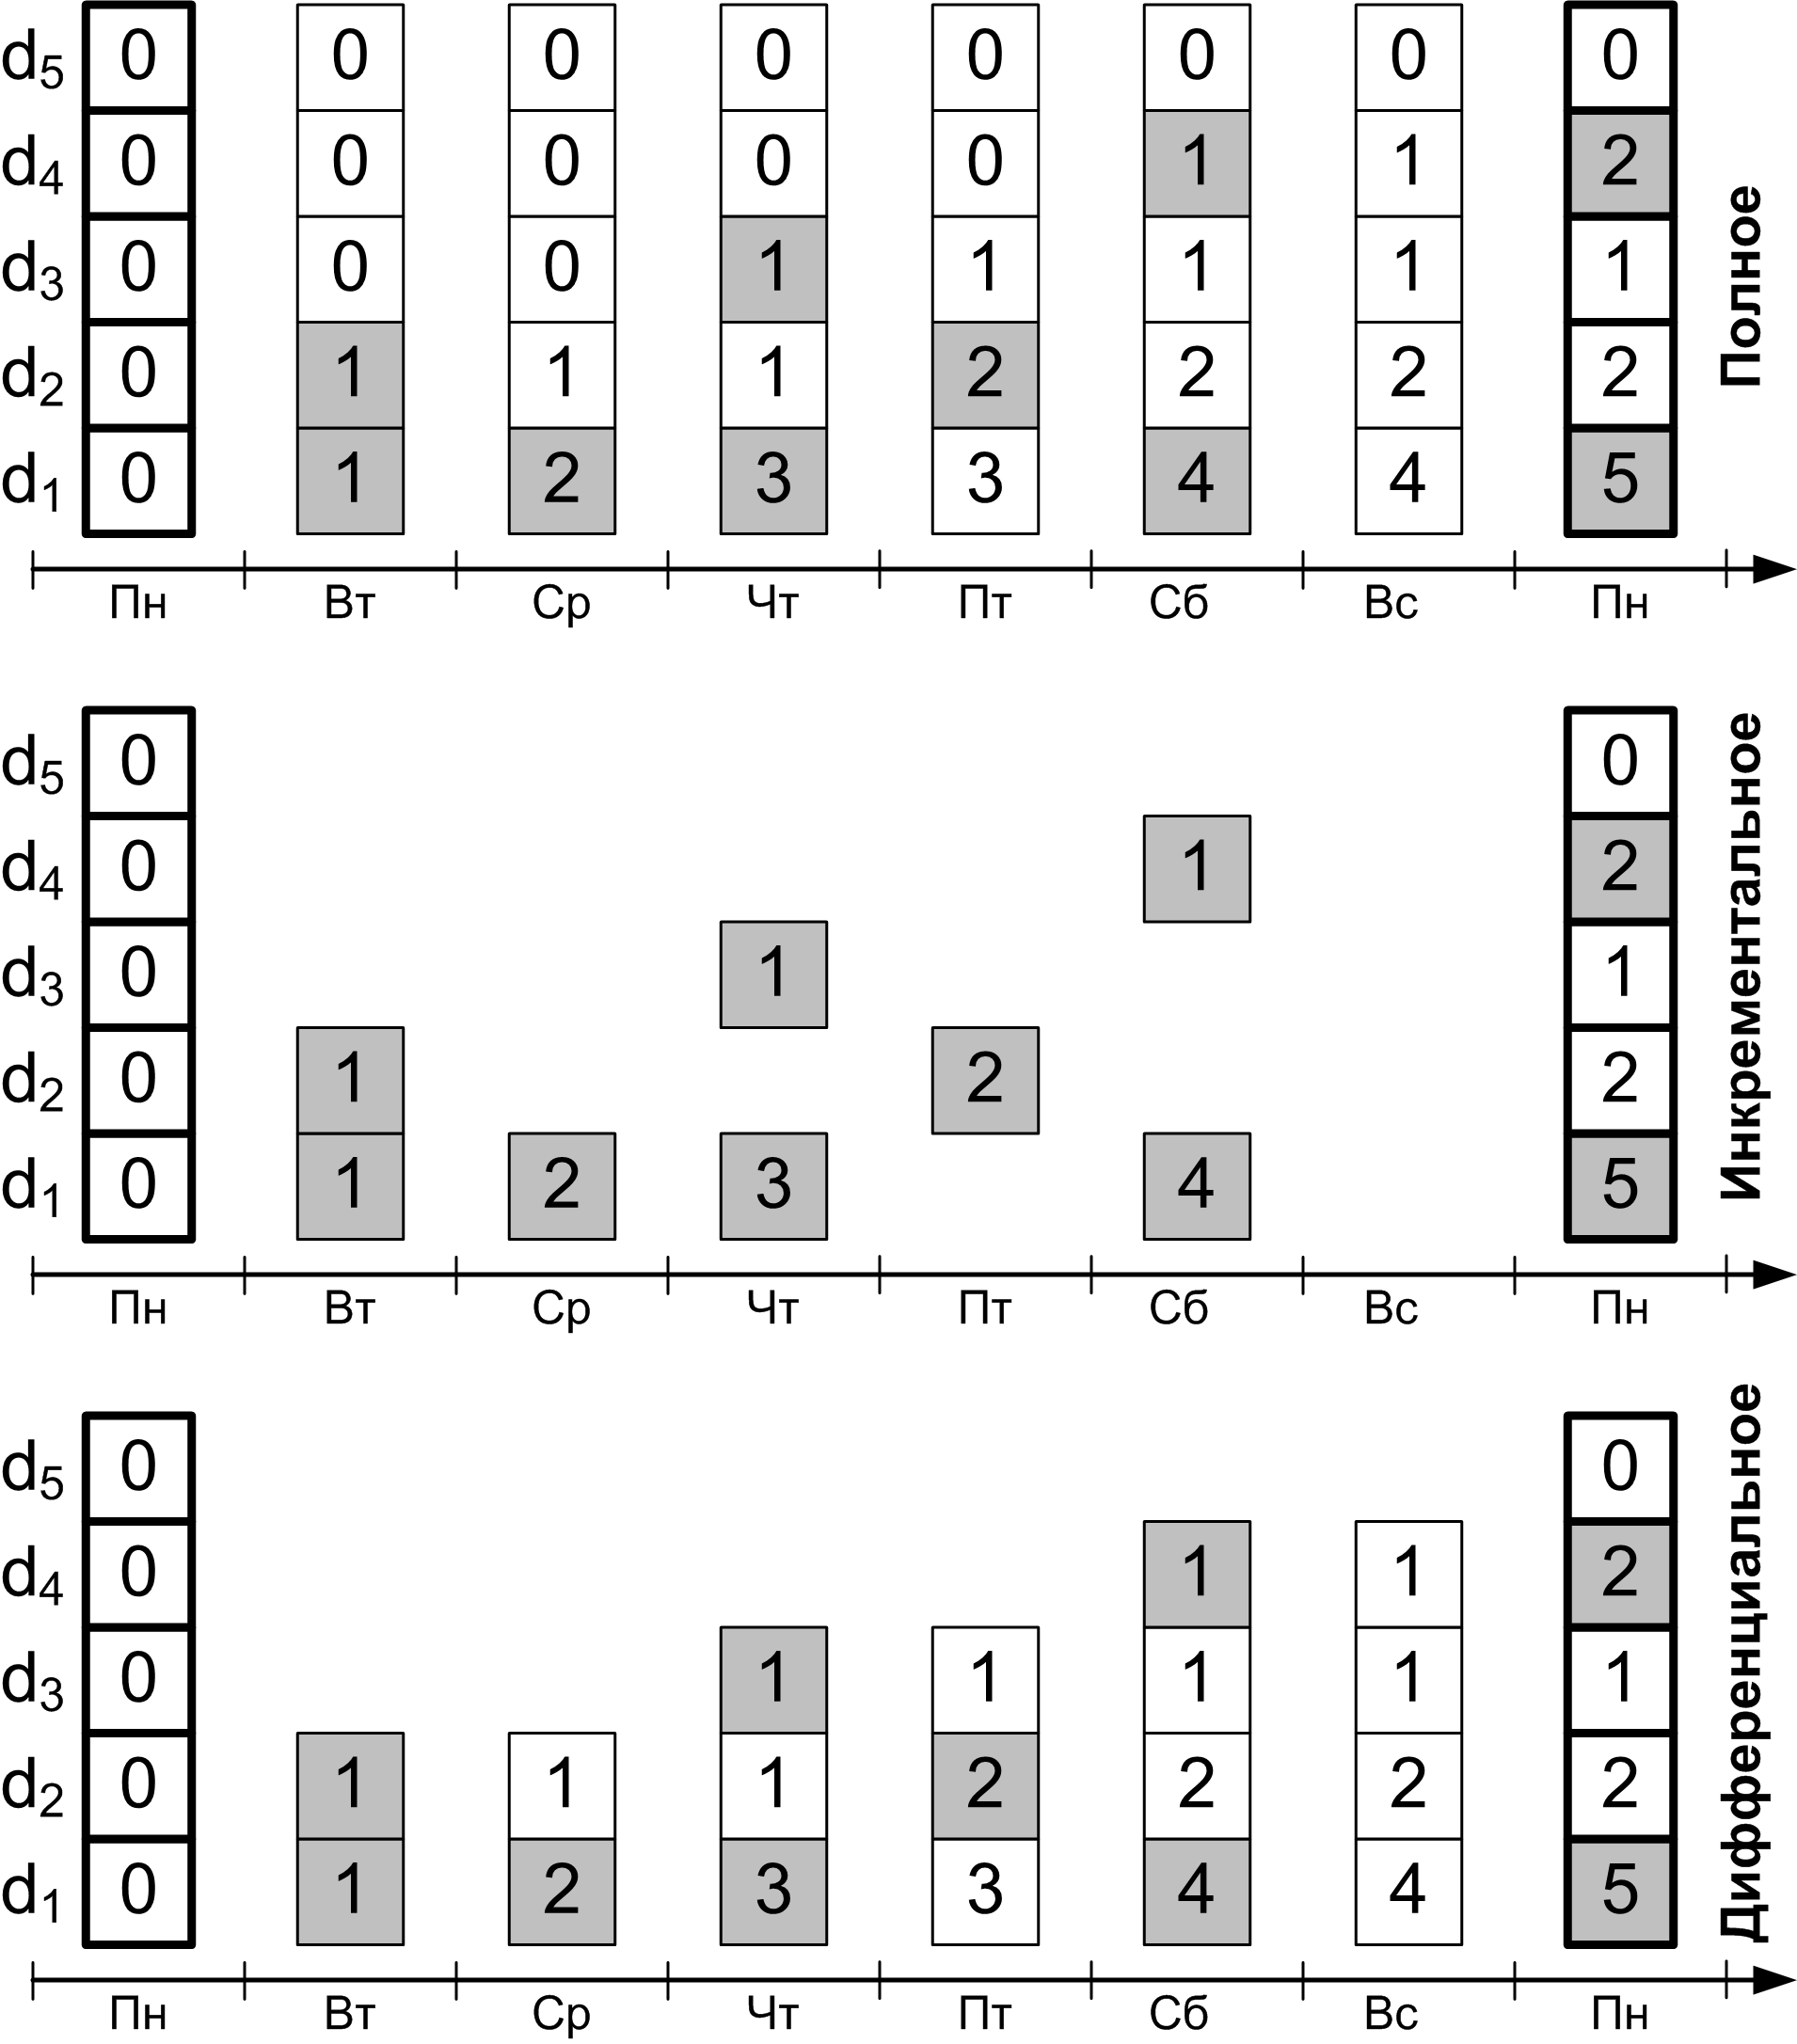
\includegraphics[height=.75\textheight]{pict/backup} }
            \mode<article>{ 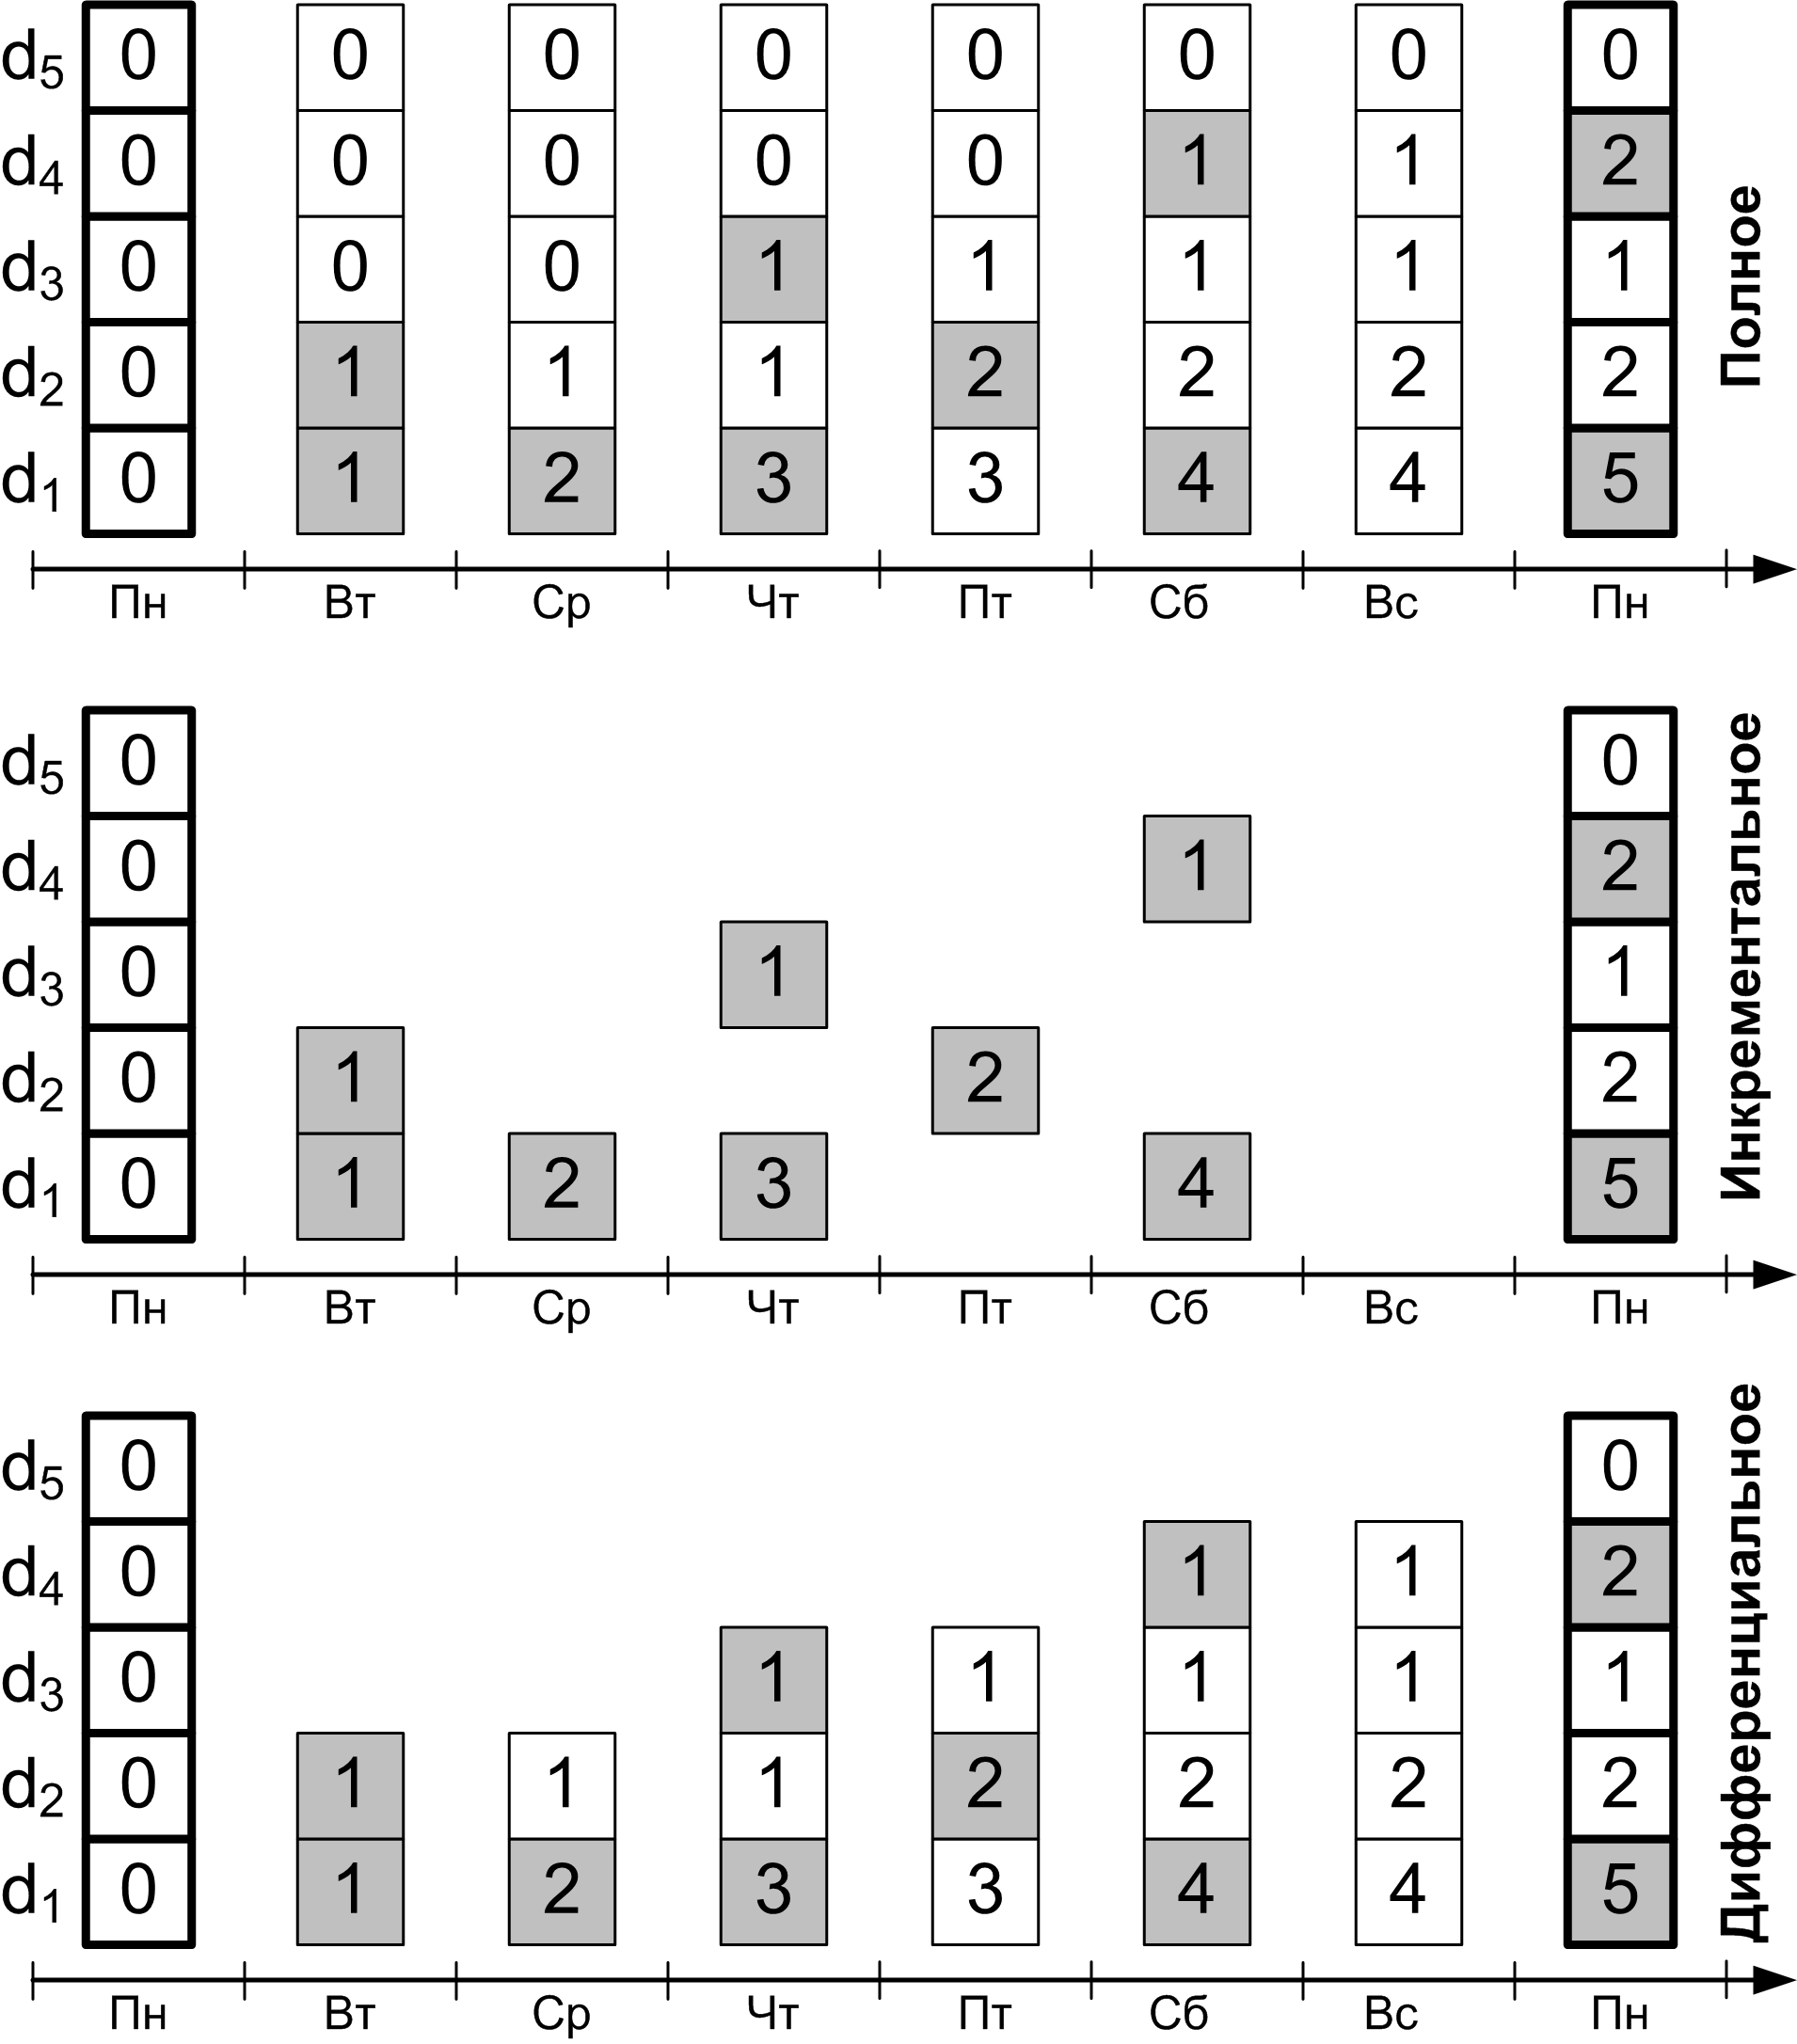
\includegraphics[width=.5\textwidth]{pict/backup} } 
            \caption{Архивирование}\label{pict:backup}
        \end{center}
    \end{figure} 
    \mode<article>{см. рис. \ref{pict:backup}}
\end{frame}

\emph{Полное}: долго делать, быстро восстанавливать, большие затраты памяти.
\emph{Инкрементальное}:быстро делать, долго восстанавливать, малые затраты памяти.
\emph{Дифференциальное}:быстро делать, быстро восстанавливать, малые затраты памяти.


\section{RAID}


\subsection{Уровни RAID}


\begin{frame}
    \frametitle{Определение}
    
    \begin{definition}%theorem, lemma, proof, corollary, example
        \alert{RAID} --- redundant array of independent/inexpensive disks. Избыточный массив независимых/недорогих жёстких дисков.
    \end{definition}
    
    Массив рассматривается системой как один накопитель. Составными элементами массива являются \alert{блочные} устройства --- диски.
    \begin{itemize}
        \item RAID 0 --- неотказоустойчивый (но высокоскоростной) массив.
        \item RAID 1 --- зеркальный массив.
        \item RAID 2 --- использует ЛБК (код Хемминга).
        \item RAID 3,4,5 --- используют чётность для защиты от одиночных неисправностей.
        \item RAID 6 --- использует чётность и арифметику полиномов для защиты от двойных неисправностей.
    \end{itemize}
\end{frame}

Реализованный аппаратно, RAID прозрачен для операционной системы и воспринимается как один накопитель. Современные операционные  системы могут моделировать работу массива программно при достаточном числе подключенных жестких дисков.

Основное назначение RAID --- увеличение скорости работы или/и повышение отказоустойчивости системы.

Выход одного или нескольких дисков из строя в составе массива не влияет на его работоспособность. Своевременно заменив вышедшие из строя диски на исправные, можно восстановить избыточность массива. Современные RAID позволяют производить такую замену <<на лету>>.

\begin{frame}
    \frametitle{RAID 0}
    
    \begin{figure}
        \begin{center}
            \mode<presentation>{ 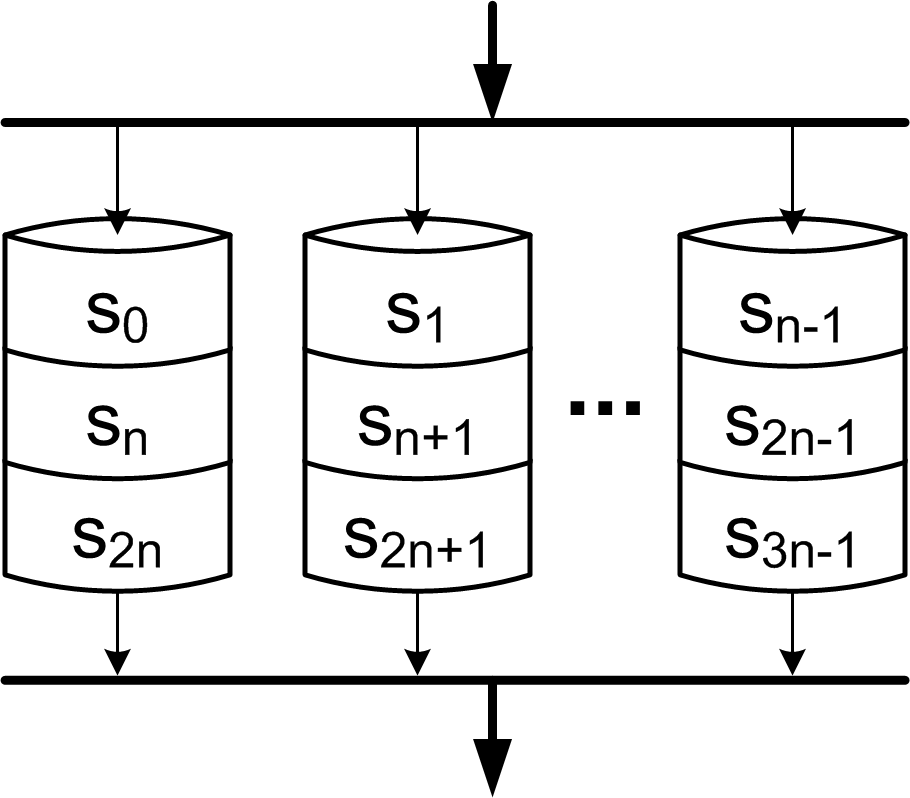
\includegraphics[height=.7\textheight]{pict/raid0} }
            \mode<article>{ 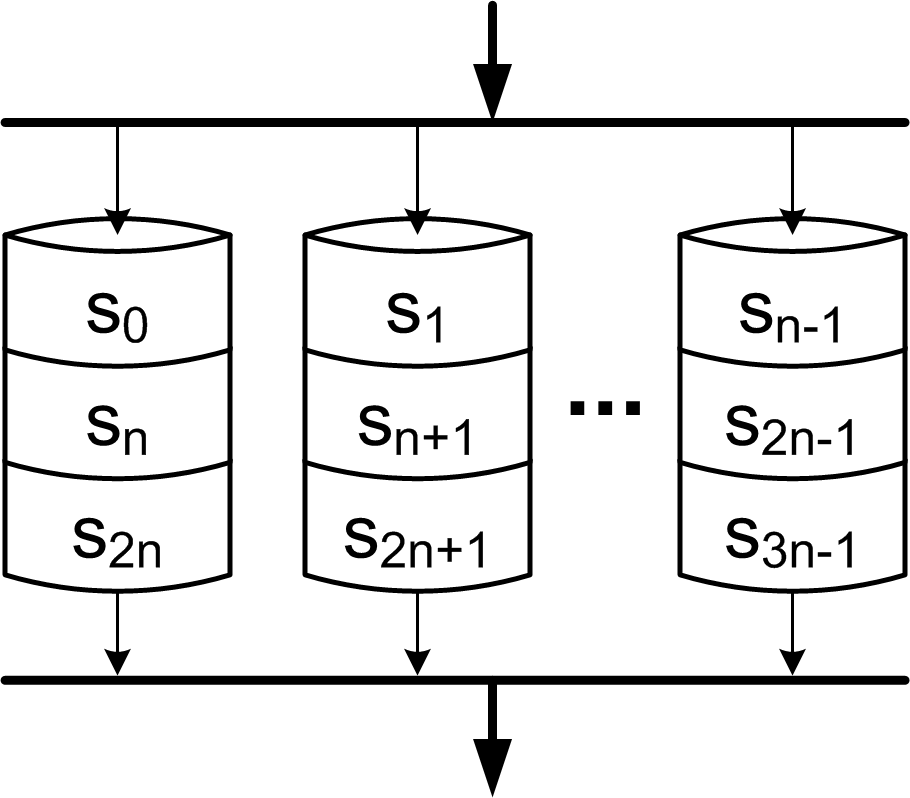
\includegraphics[width=.8\textwidth]{pict/raid0} } 
            \mode<article>{\caption{RAID 0}}\label{pict:raid0}
        \end{center}
    \end{figure} 
    \mode<article>{см. рис. \ref{pict:raid0}}
\end{frame}

Массив RAID 0 наиболее производительный и наименее защищенный из всех RAID-ов. Данные разбиваются на блоки пропорционально количеству дисков, что приводит к более высокой пропускной способности. Высокая производительность данной структуры обеспечивается \emph{параллельной} записью и отсутствием избыточного копирования. Большой блок данных будет записываться сразу на несколько дисков (посекторно), что при асинхронной работе дисков массива дает большой прирост производительности. С ростом числа дисков увеличивается и вероятность параллельной обработки нескольких запросов. 

Отказ любого диска в массиве приводит к потере данных. Этот уровень называется \emph{striping}.

Минимальное количество дисков $n=2$; Эффективность использования дискового пространства $\frac{n}{n}=1$.

Преимущества:
\begin{itemize}
    \item наивысшая производительность для приложений требующих интенсивной обработки запросов ввода/вывода.
    \item наивысшая производительность ввода/вывода для данных большого объема;
    \item простота реализации;
    \item низкая стоимость на единицу объема. 
\end{itemize}

Недостатки:
\begin{itemize}
    \item не отказоустойчивое решение;
    \item отказ одного диска влечет за собой потерю всех данных массива.
\end{itemize}


\begin{frame}
    \frametitle{RAID 1}
    
    \begin{figure}
        \begin{center}
            \mode<presentation>{ 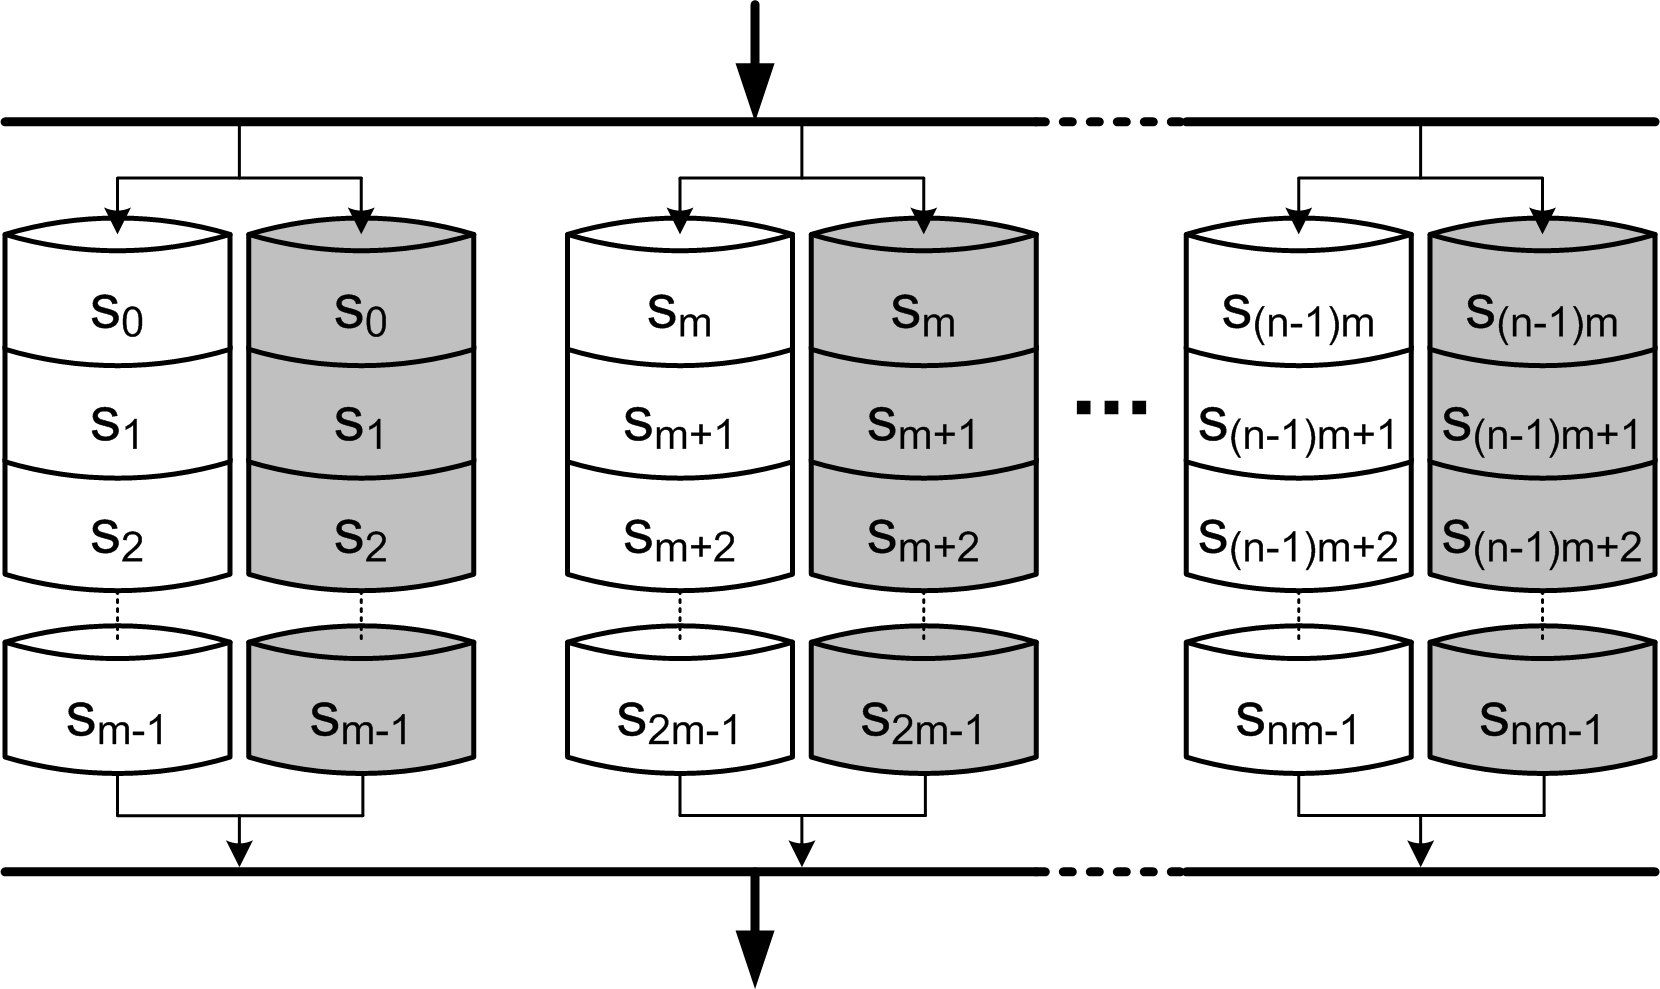
\includegraphics[height=.7\textheight]{pict/raid1} }
            \mode<article>{ 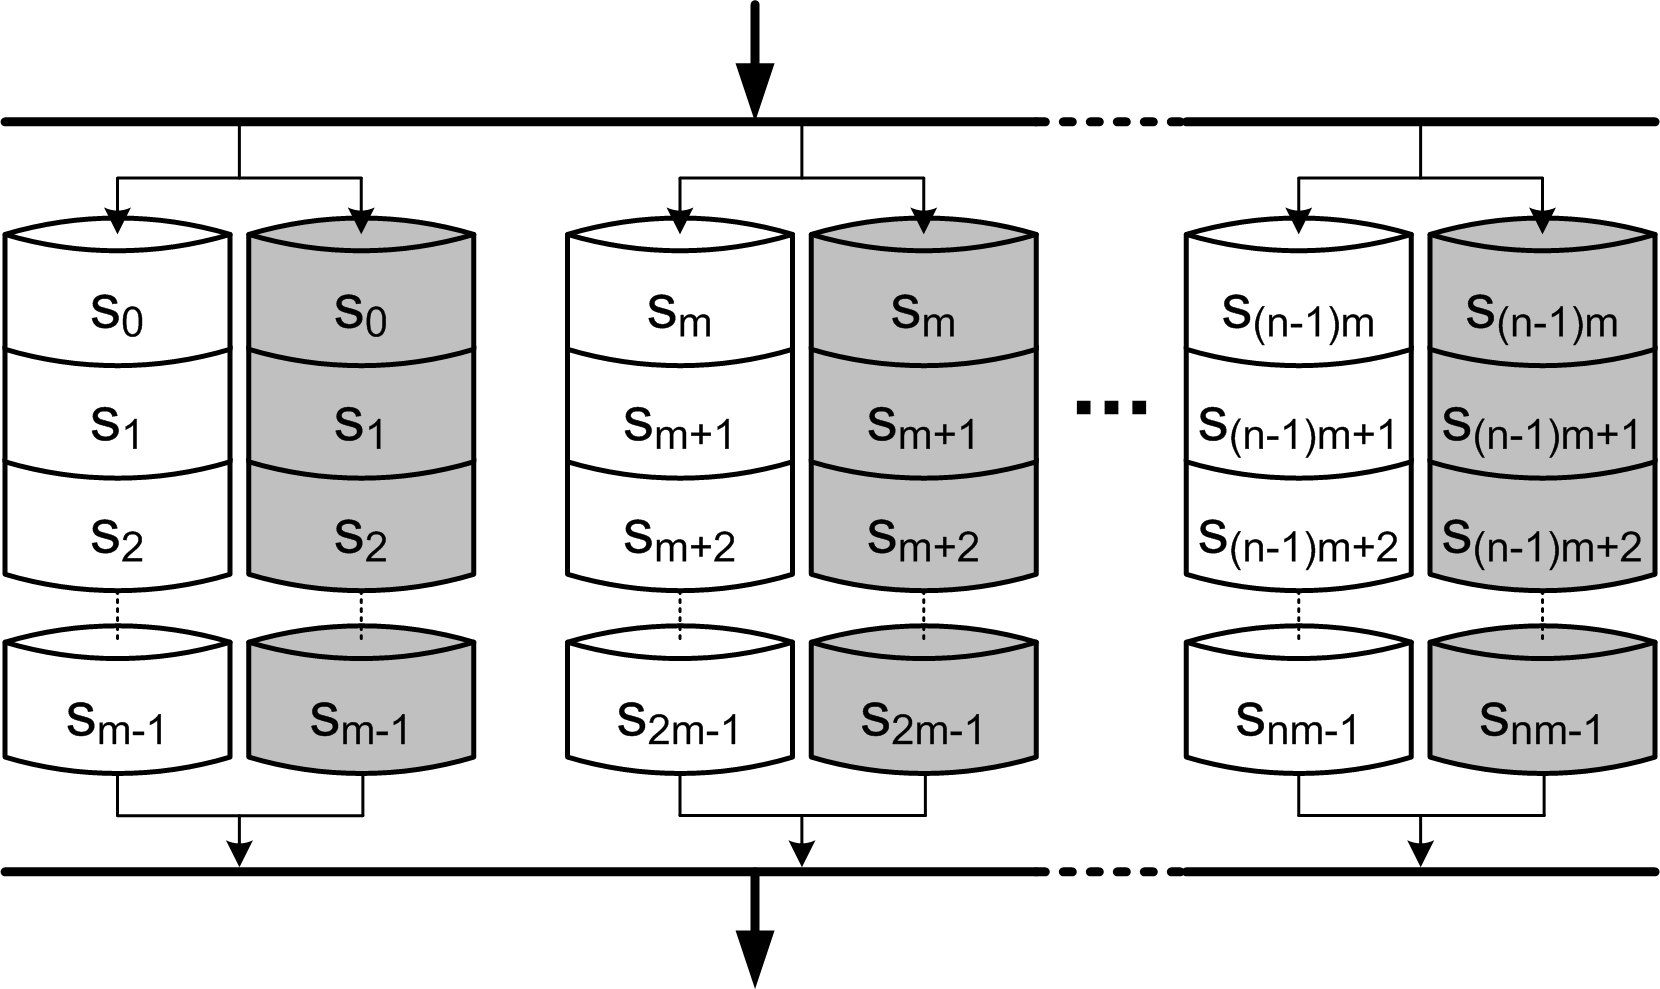
\includegraphics[width=.8\textwidth]{pict/raid1} } 
            \mode<article>{\caption{RAID 1}}\label{pict:raid1}
        \end{center}
    \end{figure} 
    \mode<article>{см. рис. \ref{pict:raid1}}
\end{frame}

RAID 1 --- mirroring (зеркалирование). Зеркальное отражение двух дисков. Избыточность структуры данного массива обеспечивает его высокую отказоустойчивость. Массив отличается высокой себестоимостью и весьма низкой производительностью. Запись больших объемов данных производится без чередования, на один диск, что сказывается на производительности.

Минимальное количество дисков: $n=2$; Эффективность использования дискового пространства: $\frac{\frac{n}{2}}{n}=\frac{1}{2}$

Преимущества:
\begin{itemize}
    \item простота реализации;
    \item простота восстановления массива в случае отказа (копирование);
    \item выход нескольких дисков из строя, если все они в разных зеркалах, не приводит к потере данынх.
\end{itemize}

Недостатки:
\begin{itemize}
    \item высокая стоимость на единицу объема. 100\% избыточность;
    \item невысокая скорость передачи данных.
\end{itemize}


\begin{frame}
    \frametitle{RAID 10}
    
    \begin{figure}
        \begin{center}
            \mode<presentation>{ 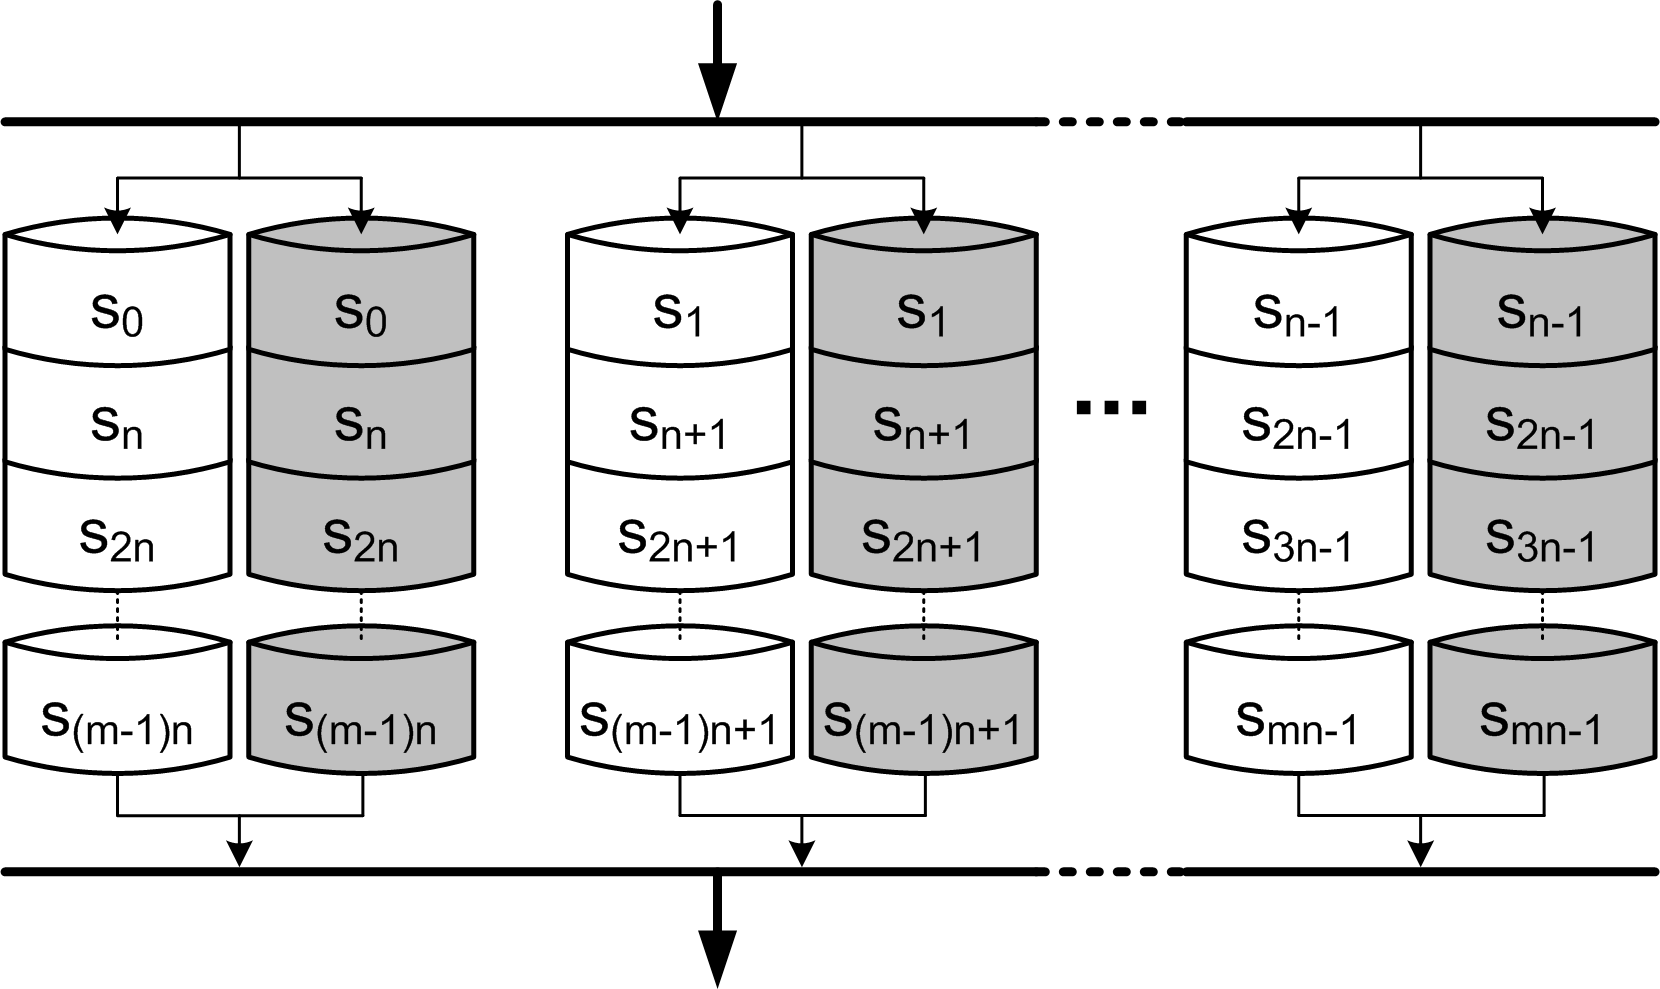
\includegraphics[height=.7\textheight]{pict/raid10} }
            \mode<article>{ 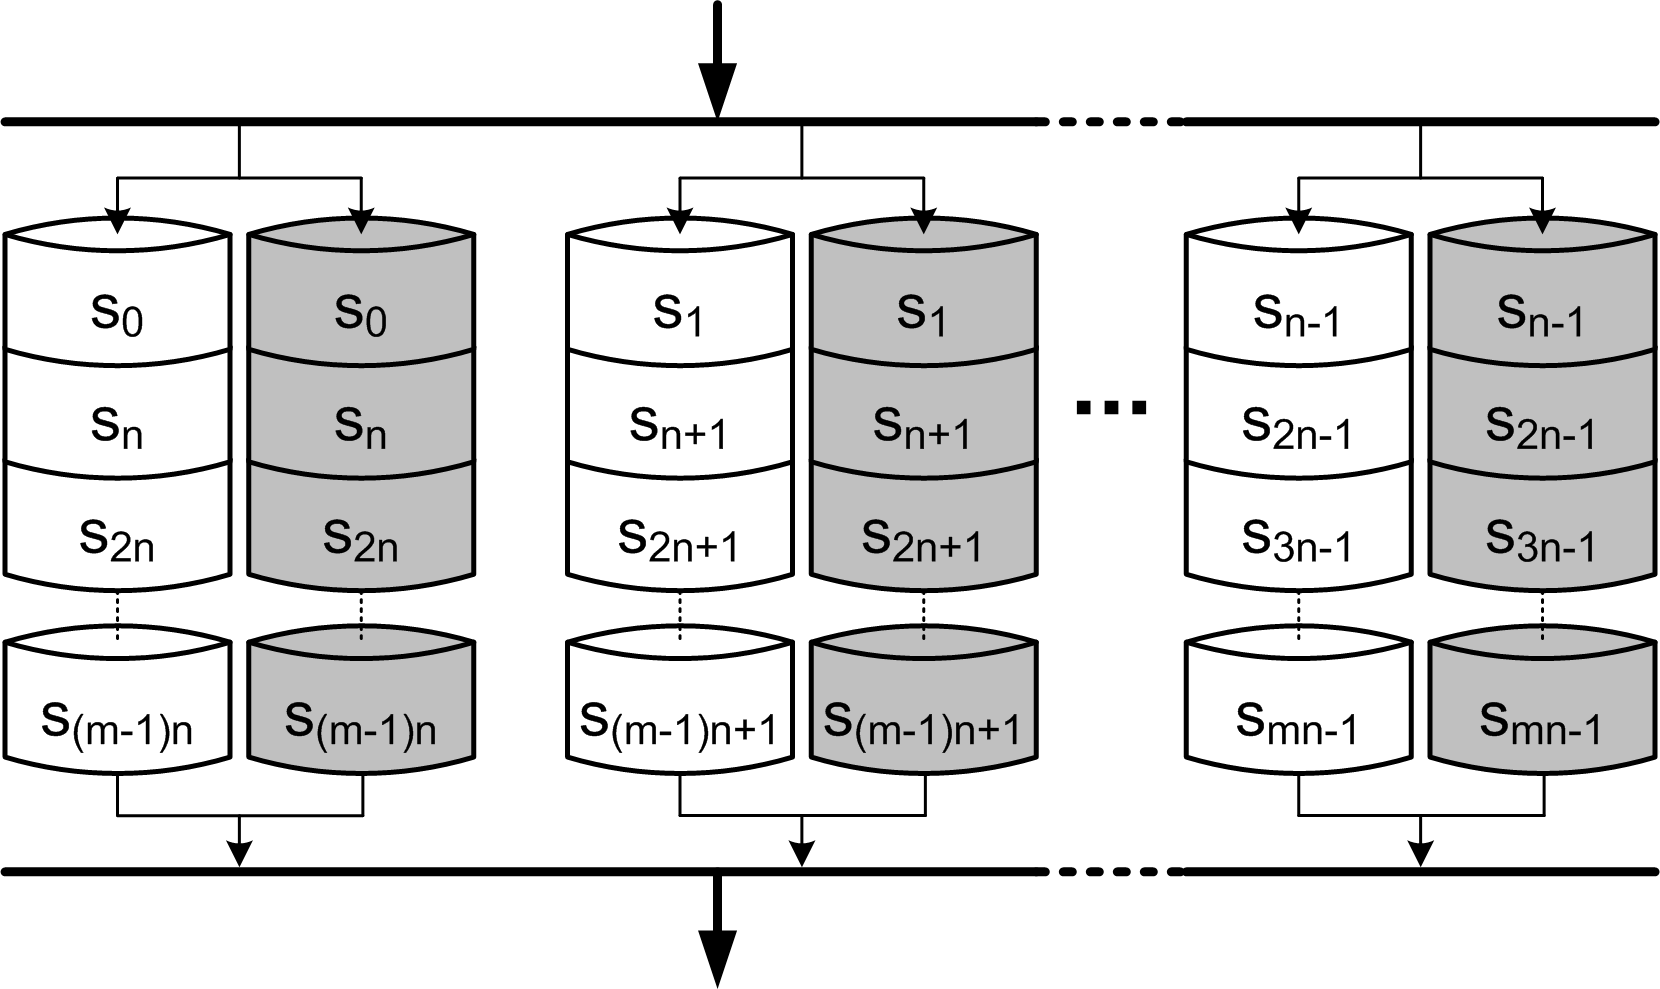
\includegraphics[width=.8\textwidth]{pict/raid10} } 
            \mode<article>{\caption{RAID 10}}\label{pict:raid10}
        \end{center}
    \end{figure} 
    \mode<article>{см. рис. \ref{pict:raid10}}
\end{frame}

RAID 10. Объединение RAID 0 и RAID 1. При всех преимуществах RAID 1 достигается производительность RAID 0. Чтение/запись с чередованием, асинхронная работа дисков массива.

Минимальное количество дисков: $n=4$; Эффективность использования дискового пространства: $\frac{\frac{n}{2}}{n}=\frac{1}{2}$

Преимущества:
\begin{itemize}
    \item простота реализации;
    \item простота восстановления массива в случае отказа (копирование);
    \item высокое быстродействие для приложений с большой интенсивностью запросов.
    \item высокое быстродействие для приложений работающих с большими объемами данных.
    \item выход нескольких дисков из строя, если все они в разных зеркалах, не приводит к потере данынх.
\end{itemize}

Недостатки:
\begin{itemize}
    \item высокая стоимость на единицу объема. 100\% избыточность;
\end{itemize}


\begin{frame}
    \frametitle{RAID 2}
    
    \begin{figure}
        \begin{center}
            \mode<presentation>{ 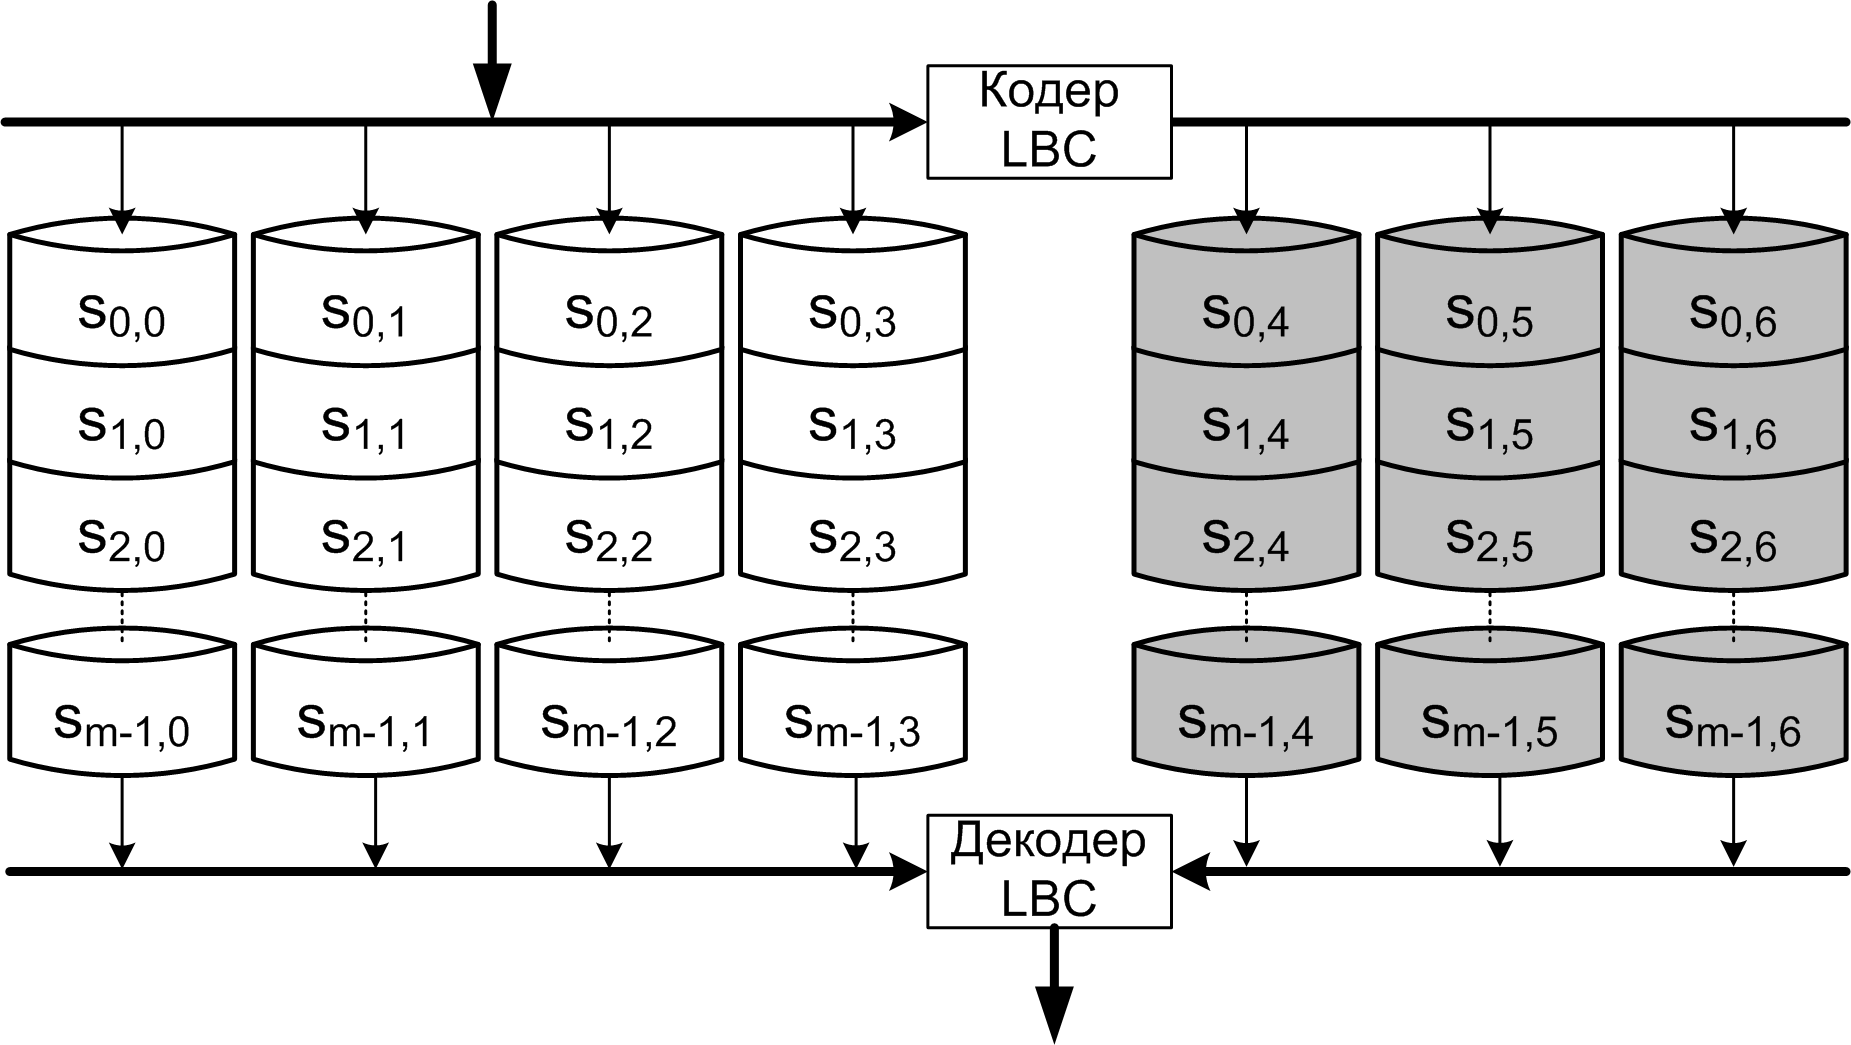
\includegraphics[height=.7\textheight]{pict/raid2} }
            \mode<article>{ 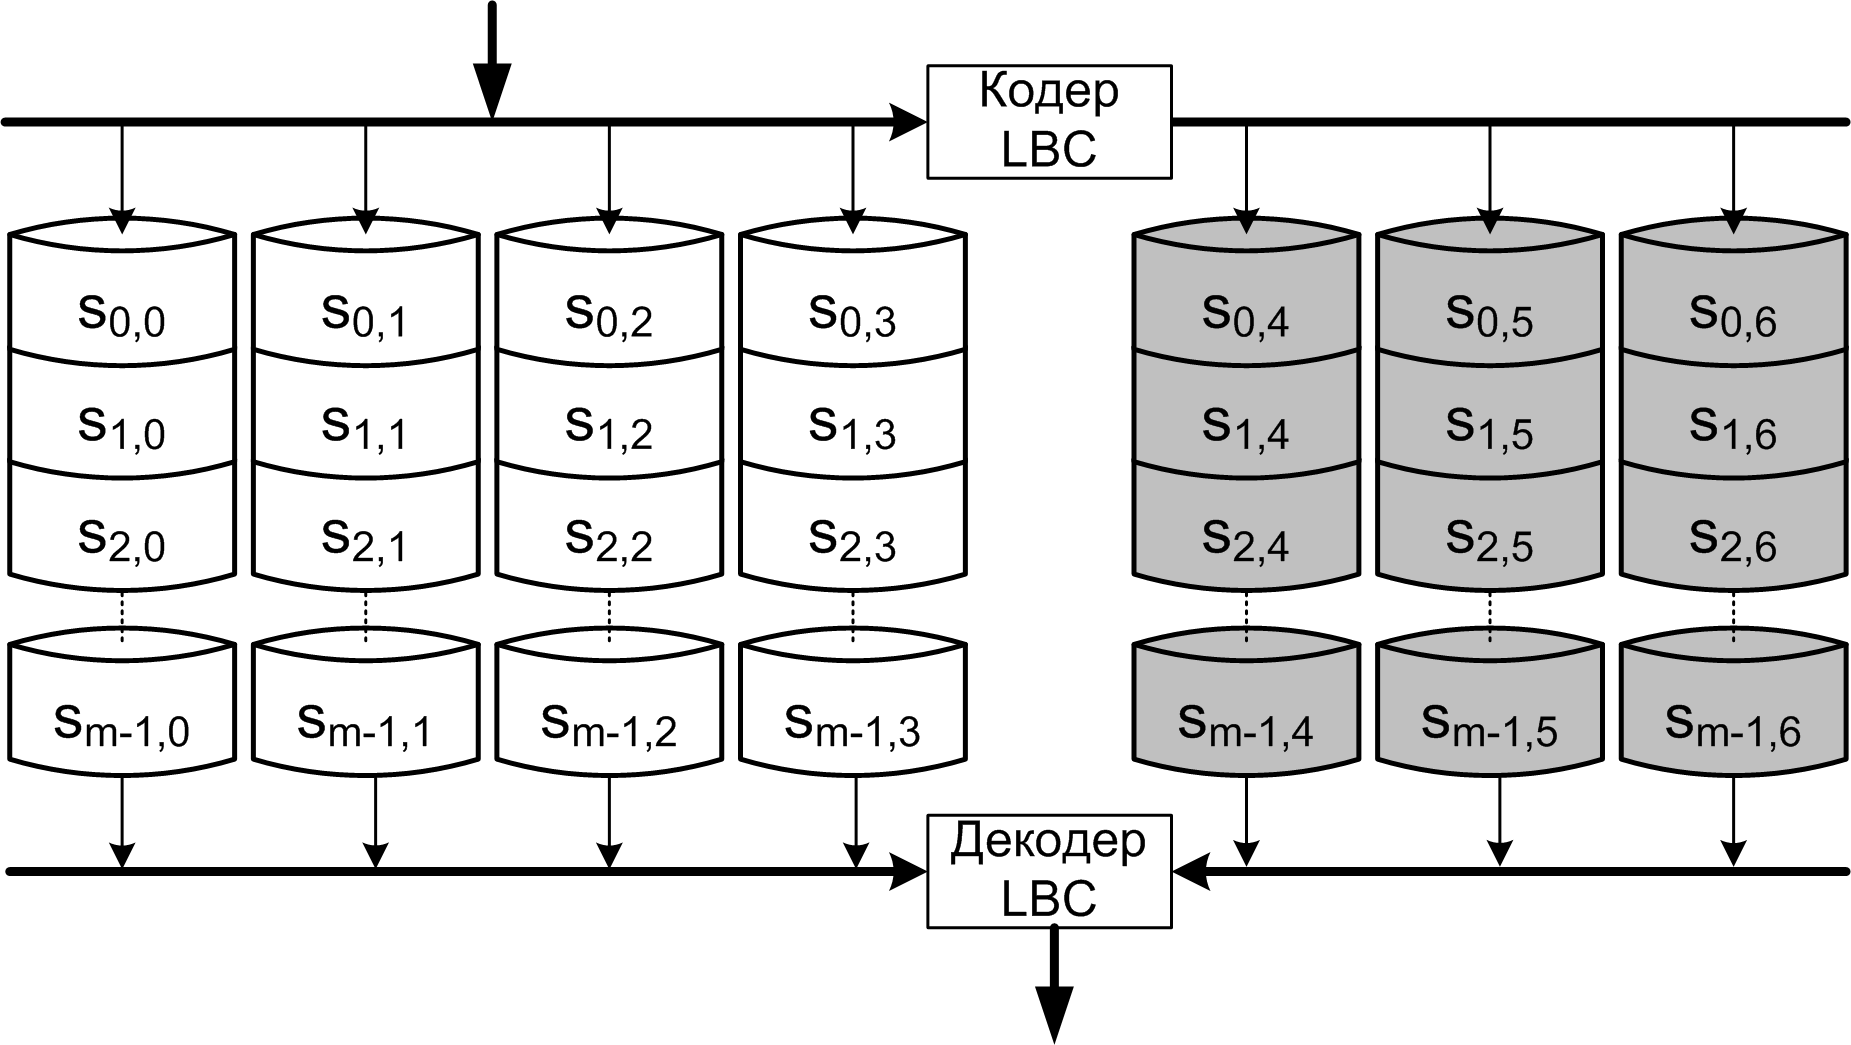
\includegraphics[width=.8\textwidth]{pict/raid2} } 
            \mode<article>{\caption{RAID 2 --- $(7,4)$-код Хемминга}}\label{pict:raid2}
        \end{center}
    \end{figure} 
    \mode<article>{см. рис. \ref{pict:raid2}}
\end{frame}


RAID 2 использует коды исправления ошибок Хемминга (Hamming Code ECC). Коды позволяют исправлять одиночные и обнаруживать двойные неисправности. Характерна синхронная работа дисков массива. Побитное расслоение, то есть каждый нулевой бит данных будет записан на нулевой диск, второй --- на второй, $i$-й на $i\pmod k$, где $k$ --- количество дисков.

Минимальное количество дисков $n=3$; Эффективность использования дискового пространства для $(n,k)$-кода $2^{n-k}\geq n+1$.

Преимущества:
\begin{itemize}
    \item быстрая коррекция ошибок <<на лету>>;
    \item высокая скорость передачи данных больших объемов;
    \item при увеличении количества дисков, накладные расходы уменьшаются;
    \item достаточно простая реализация. 
\end{itemize}

Недостатки:
\begin{itemize}
    \item высокая стоимость при малом количестве дисков;
    \item низкая скорость обработки множественных запросов (не подходит для систем ориентированных на обработку транзакций).
\end{itemize}


\begin{frame}
    \frametitle{RAID 3,4,5}
    
    Контрольная сумма вычисляется так:
    \[p=\bigoplus_{i=0}^{k-1}d_i.\]
    При выходе из строя $l$-го накопителя, его данные $d_l$ можно восстановить просуммировав осталные данные полосы: 
    \[d_l=p\oplus\left(\bigoplus_{0\leq i< k, i\neq l}d_i\right).\]
\end{frame}


\begin{frame}
    \frametitle{RAID 3}
    
    %\[p_{i,j}=\bigoplus_{l=0}^{k-1}s_{i,kj+l}\]
    
    \begin{figure}
        \begin{center}
            \mode<presentation>{ 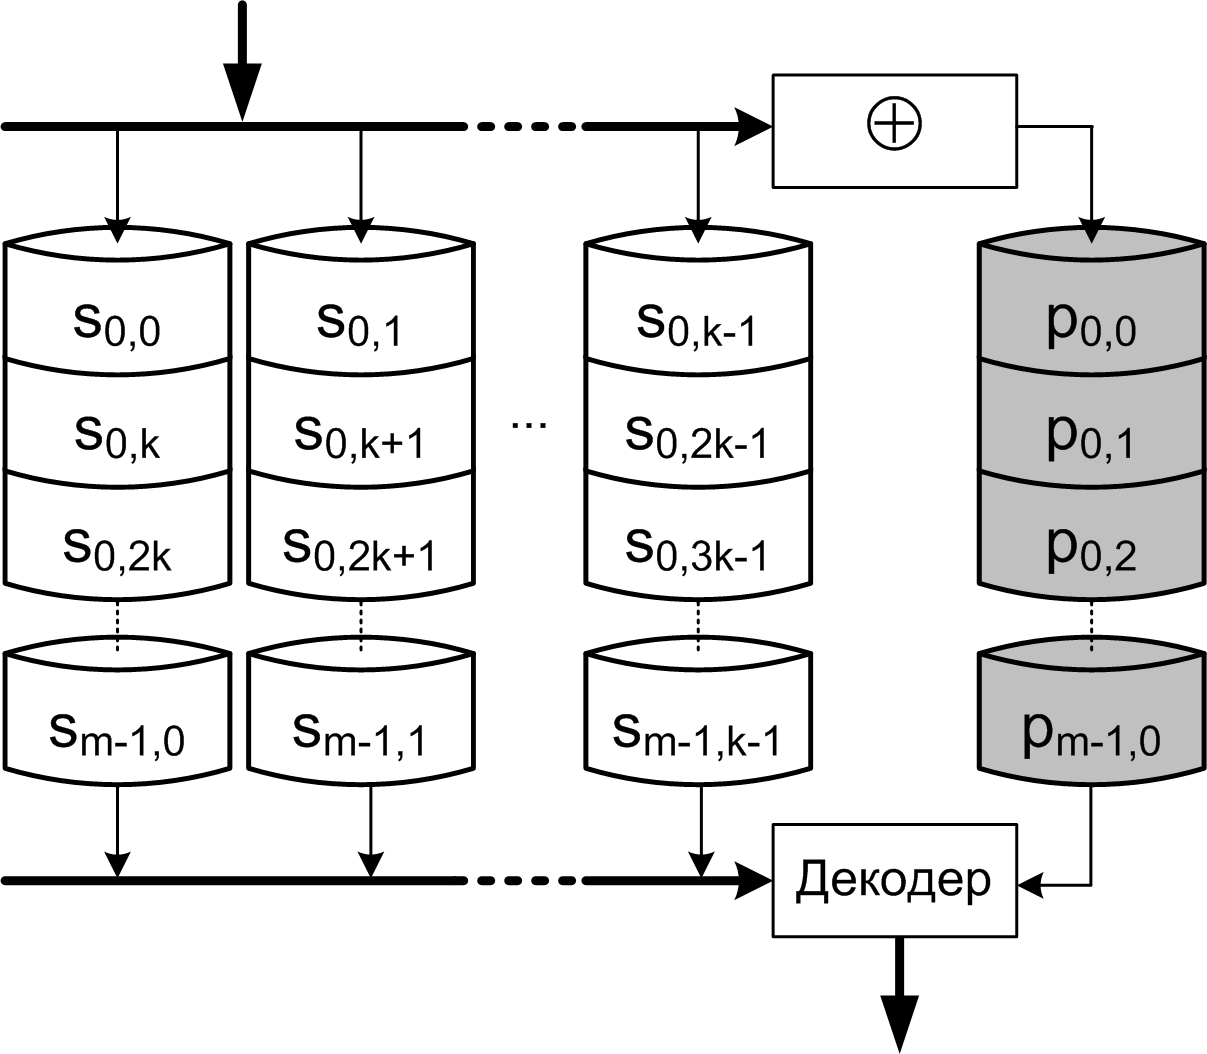
\includegraphics[height=.7\textheight]{pict/raid3} }
            \mode<article>{ 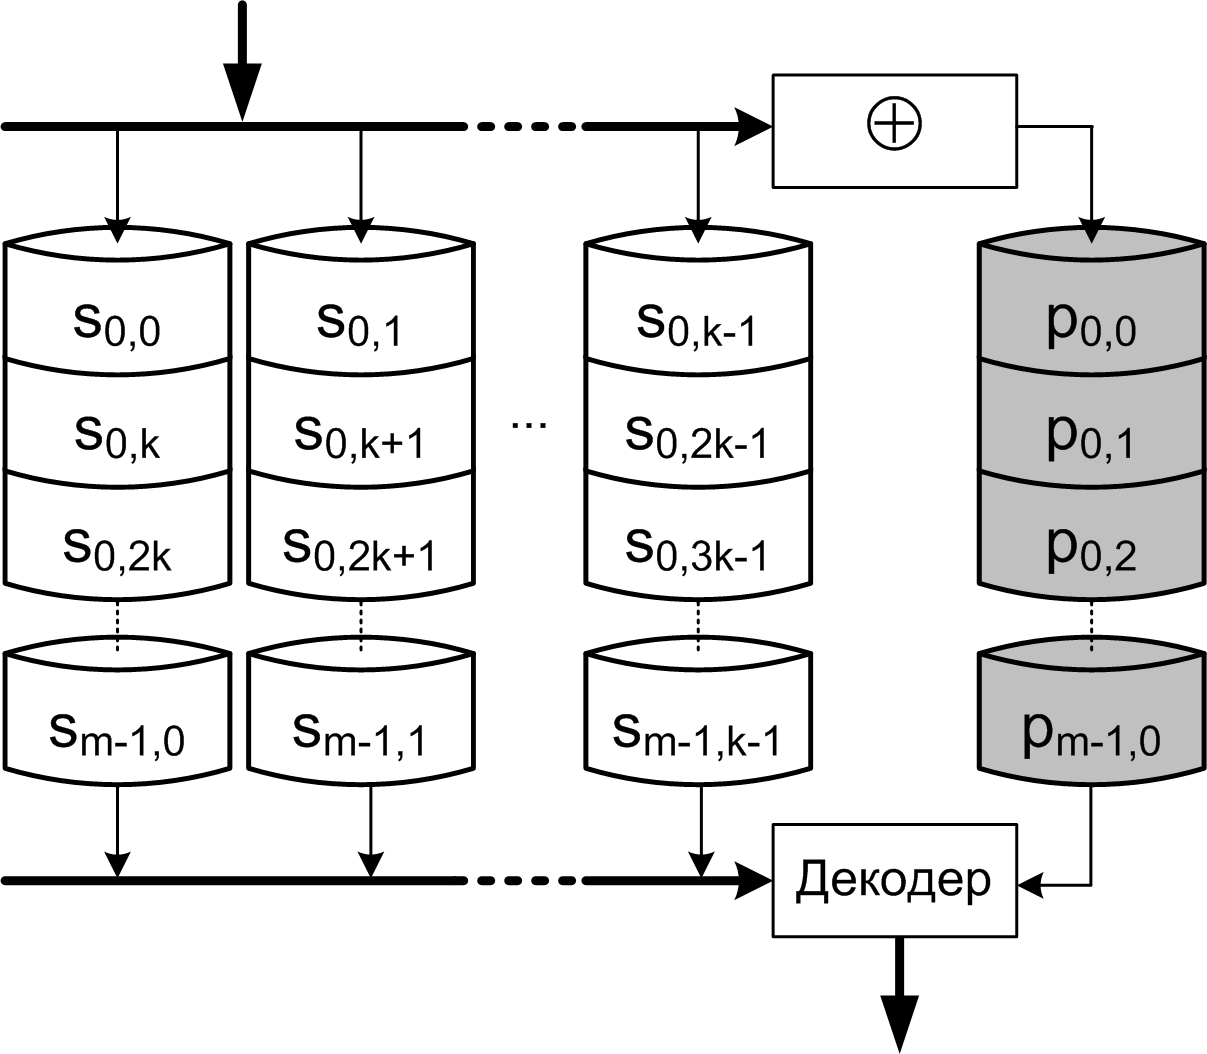
\includegraphics[width=.8\textwidth]{pict/raid3} } 
            \mode<article>{\caption{RAID 3}}\label{pict:raid3}
        \end{center}
    \end{figure} 
    \mode<article>{см. рис. \ref{pict:raid3}}
\end{frame}

\[p_{i,j}=\bigoplus_{l=0}^{k-1}s_{i,kj+l}\]

Структура массива RAID 3 такова: в массиве из $n$ дисков данные разбиваются на блоки размером 1 байт и распределяются по $k = n-1$ дискам, (т.е. каждый следующий байт последовательности хранится на другом диске. нулевой диск из n будет хранить байты $0$, $k$, $2k$, $3k$, и т.д.) а еще один диск используется для хранения блоков четности. Характерна синхронная работа дисков.

Минимальное количество дисков: $n=3$; Эффективность использования дискового пространства: $\frac{n-1}{n}$
Преимущества:
\begin{itemize}
    \item очень высокая скорость передачи данных большого объема (например в задачах обработки видео);
    \item отказ диска мало влияет на скорость работы массива;
    \item малые накладные расходы для реализации избыточности. 
\end{itemize}

Недостатки:
\begin{itemize}
    \item низкая производительность при большой интенсивности запросов данных небольшого объема.
\end{itemize}


\begin{frame}
    \frametitle{RAID 4}
    
    %\[p_{i}=\bigoplus_{l=0}^{k-1}s_{kj+l}\]
    
    \begin{figure}
        \begin{center}
            \mode<presentation>{ 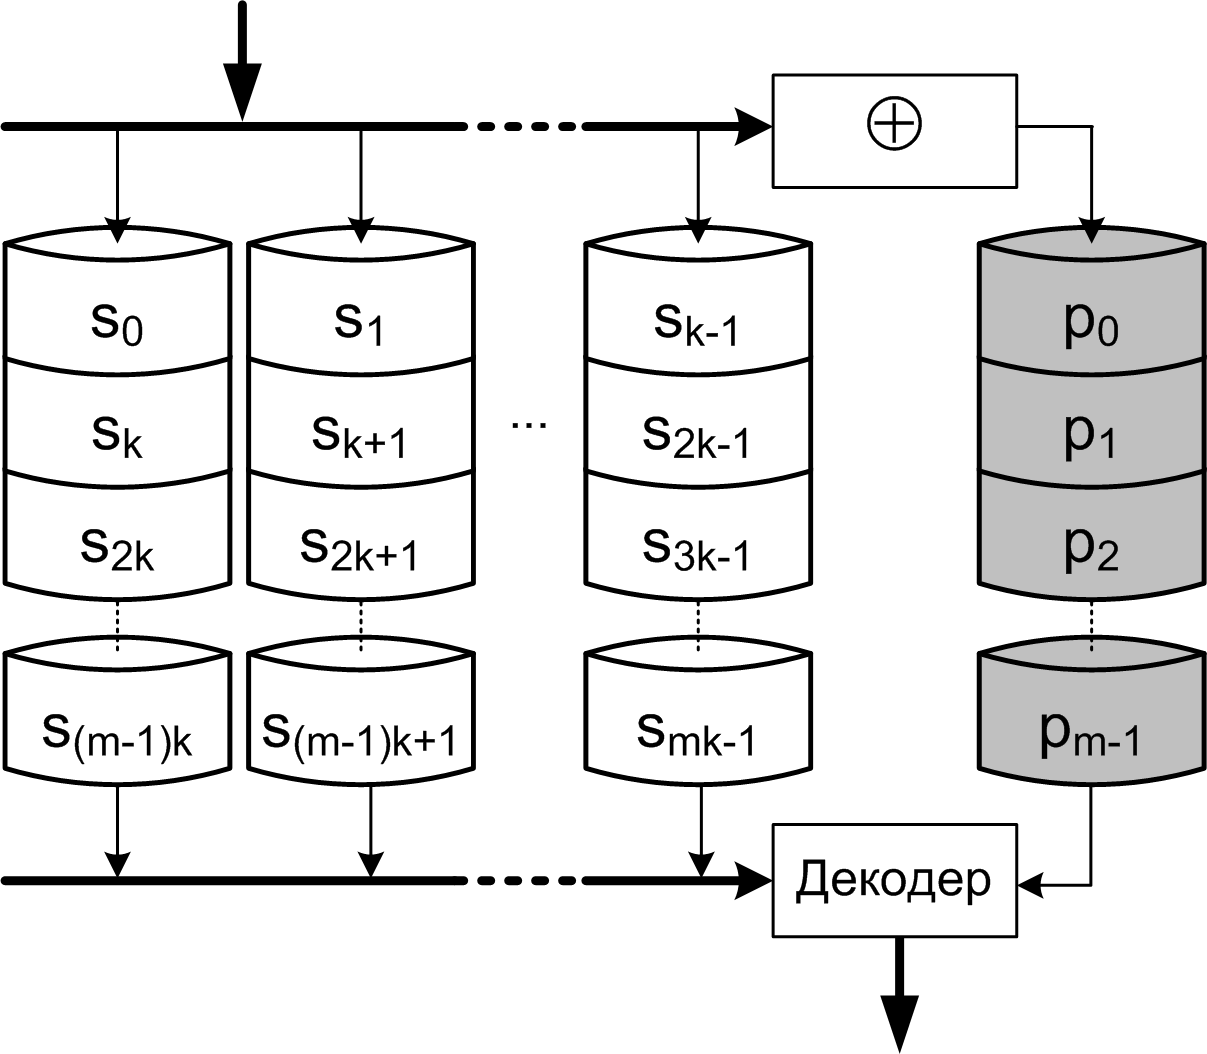
\includegraphics[height=.7\textheight]{pict/raid4} }
            \mode<article>{ 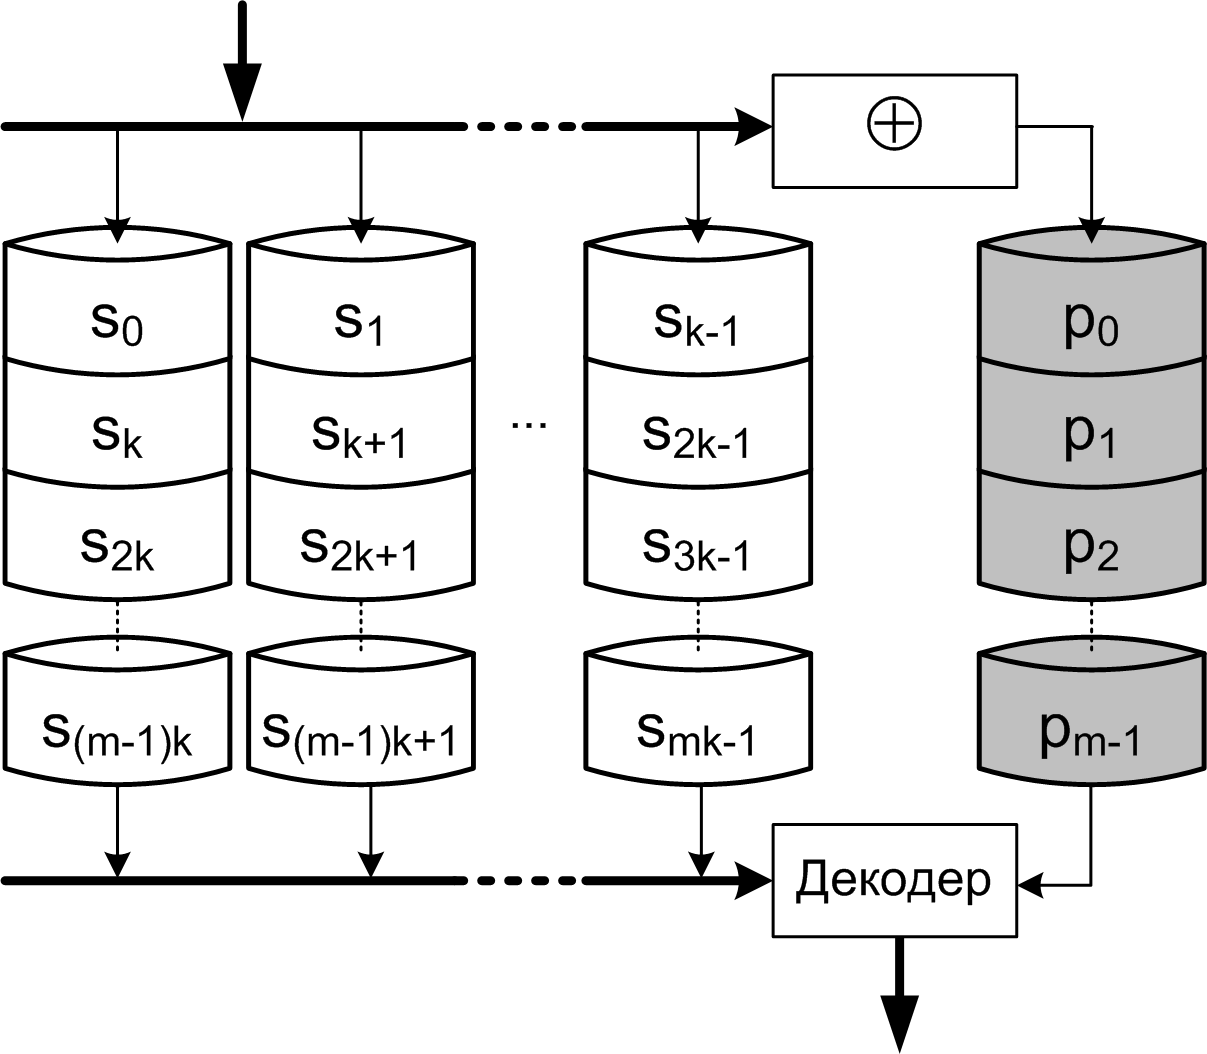
\includegraphics[width=.8\textwidth]{pict/raid4} } 
            \mode<article>{\caption{RAID 4}}\label{pict:raid4}
        \end{center}
    \end{figure} 
    \mode<article>{см. рис. \ref{pict:raid4}}
\end{frame}

\[p_{i}=\bigoplus_{l=0}^{k-1}s_{kj+l}\]

Отказоустойчивый массив независимых дисков с разделяемым диском четности (Independent Data disks with shared Parity disk).

Минимальное количество дисков: $n=3$; Эффективность использования дискового пространства: $\frac{n-1}{n}$.

RAID 4 имеет схожую структуру с RAID 3, однако отличие состоит в том, что в RAID 4 расслоение данных происходит на уровне секторов, а не на уровне байтов. У RAID 4 более высокая производительность передачи малых объемов данных за счет распараллеливания, при котором имеется возможность выполнять более одного обращения по I/O контуру одновременно.

\[p=\bigoplus_{i=0}^{k-1}s_i\] при выходе из строя $l$-го диска, $s_l$ восстанавливается как сумма оставшихся $s_i$ и $p$:
\[s_l=p\oplus \bigoplus_{0\leq i<k,i\neq l}s_i\]

Казалось бы при записи $s'_i$, для того чтобы сформировать контрольную полосу нужно считать данные со всех $k$ дисков. Но нет, достаточно считать данные с диска, на который идет запись: $s_i$, считать данные контрольной полосы $p$ и записать $p'=p\oplus s_i \oplus s'_i$.

Диск, содержащий данные контрольной суммы $p$ является узким местом при параллельных операциях записи: запись контрольных данных приходится осуществлять последовательно.

Преимущества:
\begin{itemize}
    \item высокая скорость чтения данных больших объемов;
    \item высокая производительность при большой интенсивности запросов чтения данных;
    \item малые накладные расходы для реализации избыточности. 
\end{itemize}

Недостатки:
\begin{itemize}
    \item низкая производительность при записи данных;
    \item асимметричность быстродействия относительно чтения и записи.
\end{itemize}


\begin{frame}
    \frametitle{RAID 5}
    
    \begin{figure}
        \begin{center}
            \mode<presentation>{ 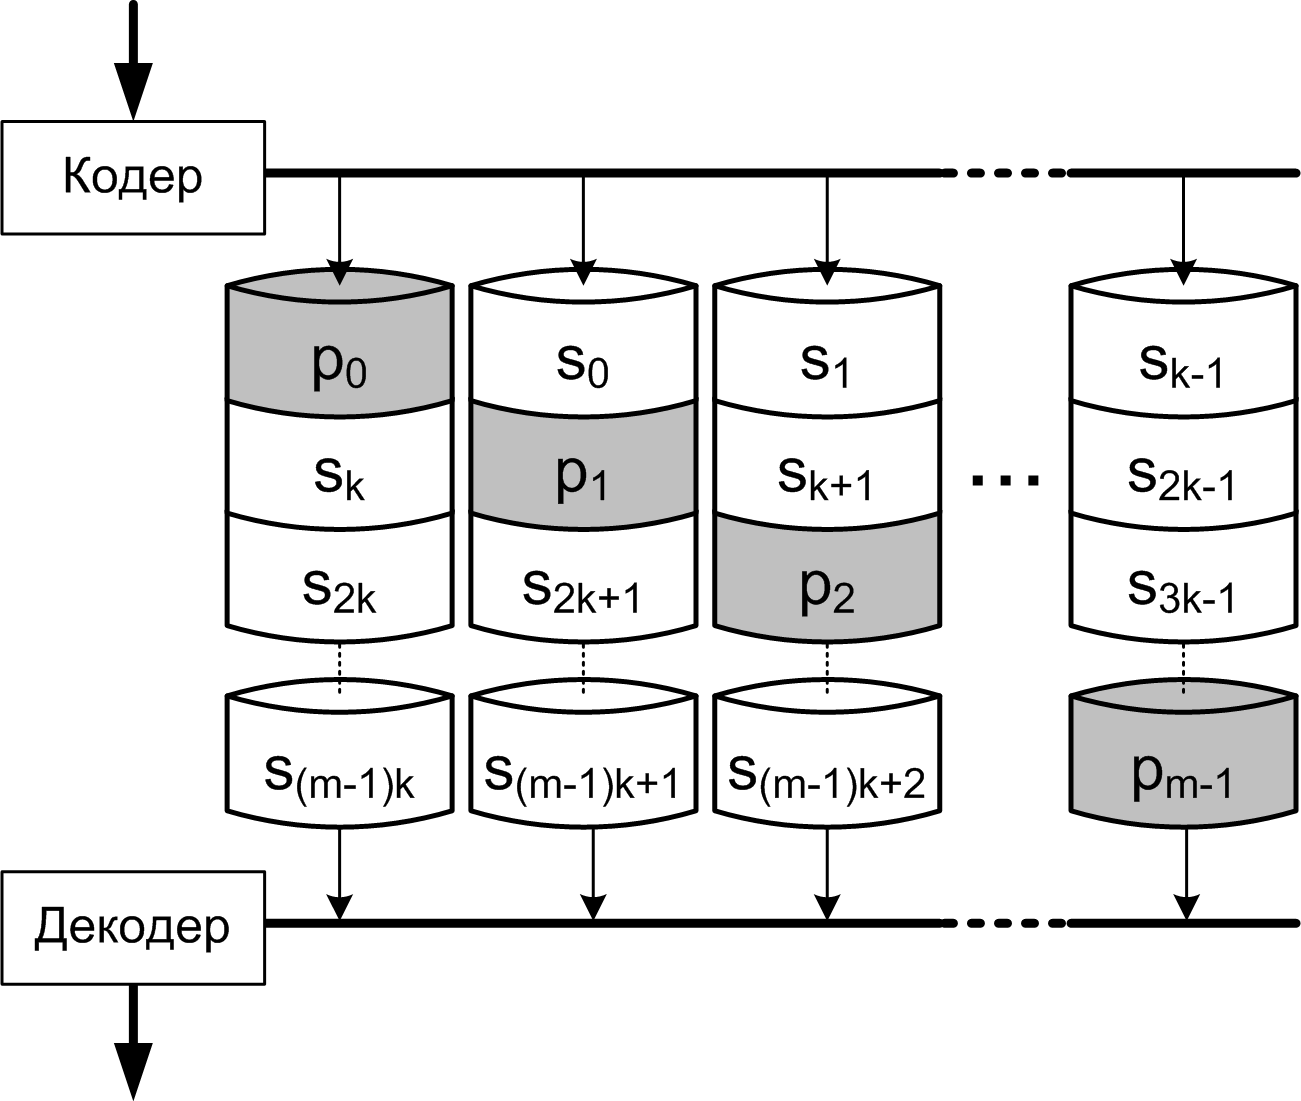
\includegraphics[height=.7\textheight]{pict/raid5} }
            \mode<article>{ 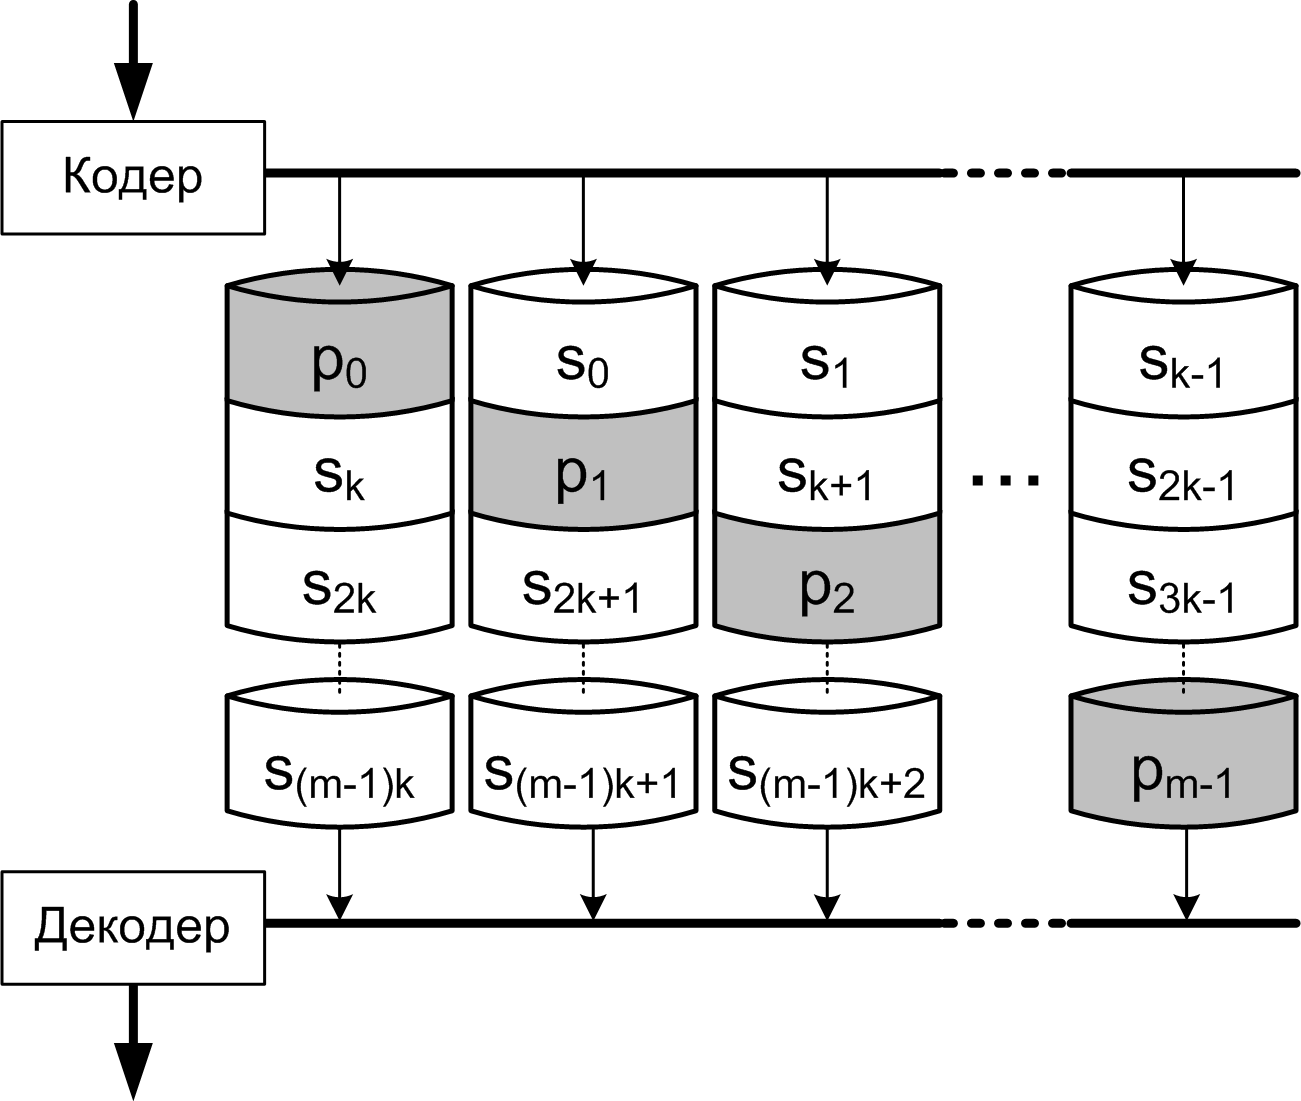
\includegraphics[width=.8\textwidth]{pict/raid5} } 
            \mode<article>{\caption{RAID 5}}\label{pict:raid5}
        \end{center}
    \end{figure} 
    \mode<article>{см. рис. \ref{pict:raid5}}
\end{frame}


Отказоустойчивый массив независимых дисков с распределенной четностью (Independent Data disks with distributed parity blocks).

RAID 5 упоминается как striping с распределенной контрольной суммой. В отличие от RAID 4 в RAID 5 контрольная сумма распределяется среди дисков. Это изменение позволяет увеличить производительность записи небольших объемов данных в многозадачных системах. Поскольку данные четности распределяются среди дисков, скорость выполнение процесса чтения имеет тенденцию быть значительно ниже чем скорость чтения у RAID 4 уровня.

Минимальное количество дисков $n=3$; Эффективность использования дискового пространства: $\frac{n-1}{n}$.

Преимущества:
\begin{itemize}
    \item высокая скорость записи данных;
    \item достаточно высокая скорость чтения данных;
    \item высокая производительность при большой интенсивности запросов чтения/записи данных;
    \item малые накладные расходы для реализации избыточности. 
\end{itemize}

Недостатки:
\begin{itemize}
    \item скорость чтения данных ниже, чем в RAID 4;
    \item низкая скорость чтения/записи данных малого объема при единичных запросах;
    \item достаточно сложная реализация;
    \item восстановление данных происходит медленно.
\end{itemize}


\begin{frame}
    \frametitle{RAID 6}
    
    В RAID 6 одна из контрольных сумм вычисляется так же как и в RAID 5:
    \[ p=\bigoplus_{j=0}^{k-1}s_{j}. \]
    
    Для вычисления второй контрольной суммы используется арифметика полиномов\footnote{Например, используют поле $\mathbb{F}_2[X]/(X^8+X^4+X^3+X^2+1)$, в котором \alert{примитивным} элементом является полином $X$.}:
    \[ q=\bigoplus_{j=0}^{k-1}g^js_{j}, \]
    где $g$ --- примитивный элемент.
\end{frame}


\begin{frame}
    \frametitle{RAID 6}
    
    \begin{figure}
        \begin{center}
            \mode<presentation>{ 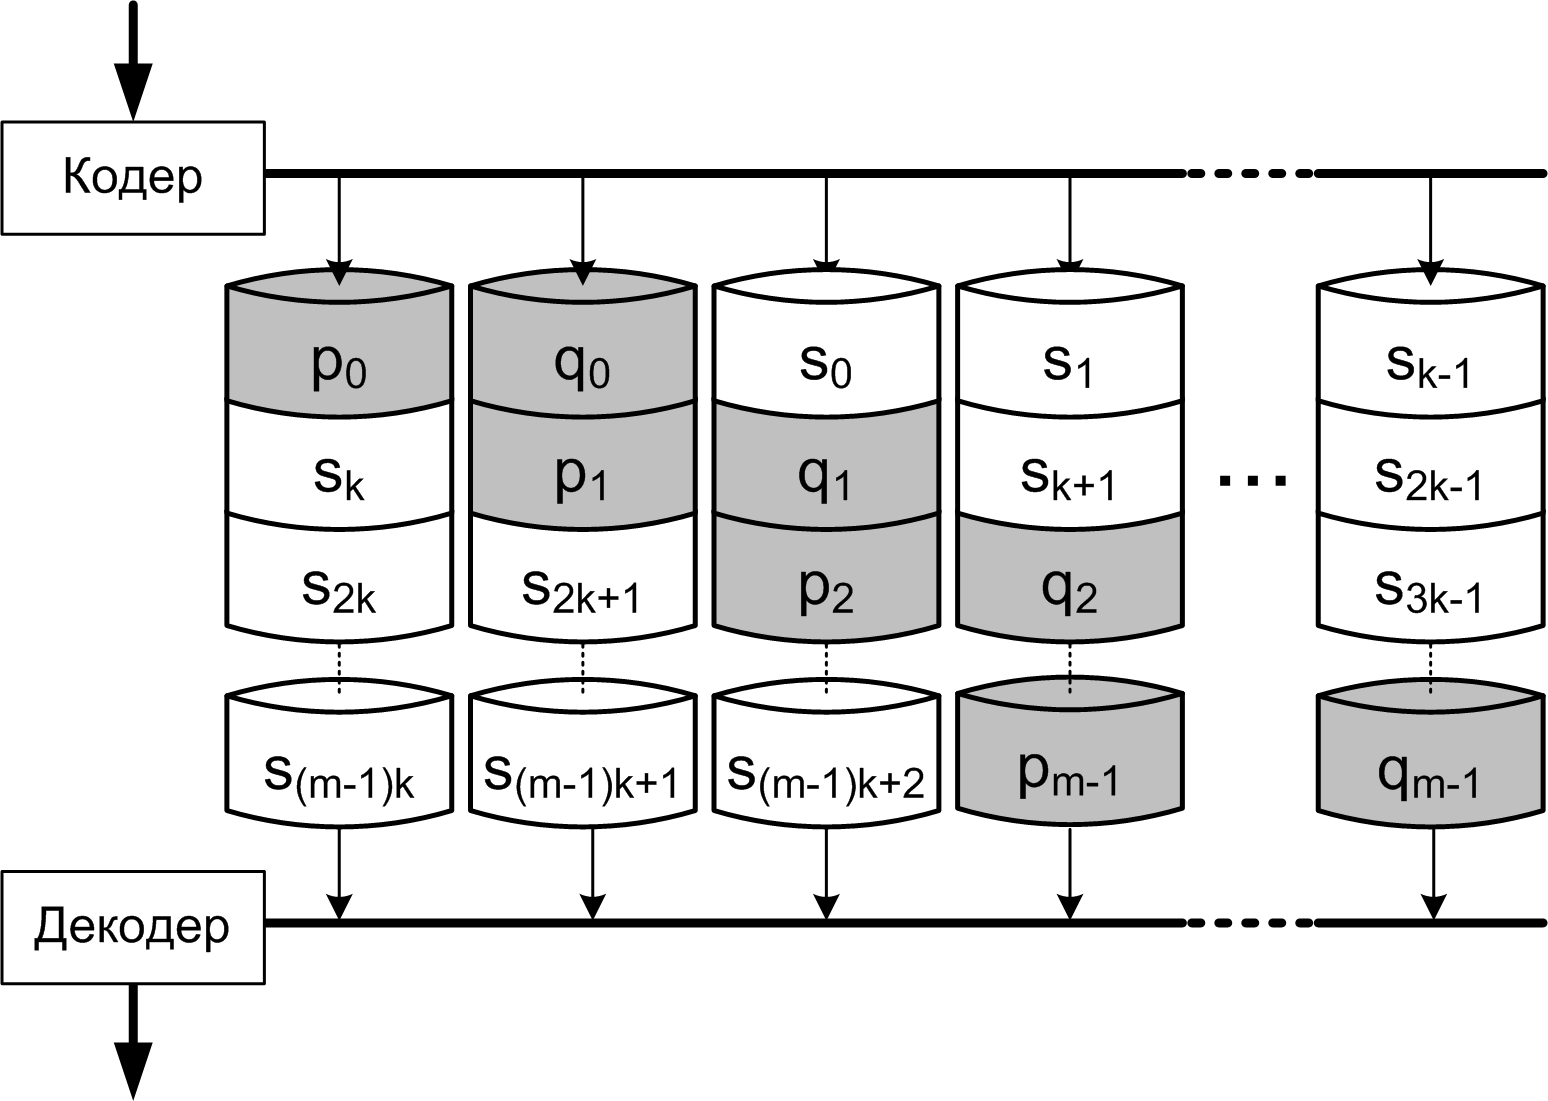
\includegraphics[height=.7\textheight]{pict/raid6} }
            \mode<article>{ 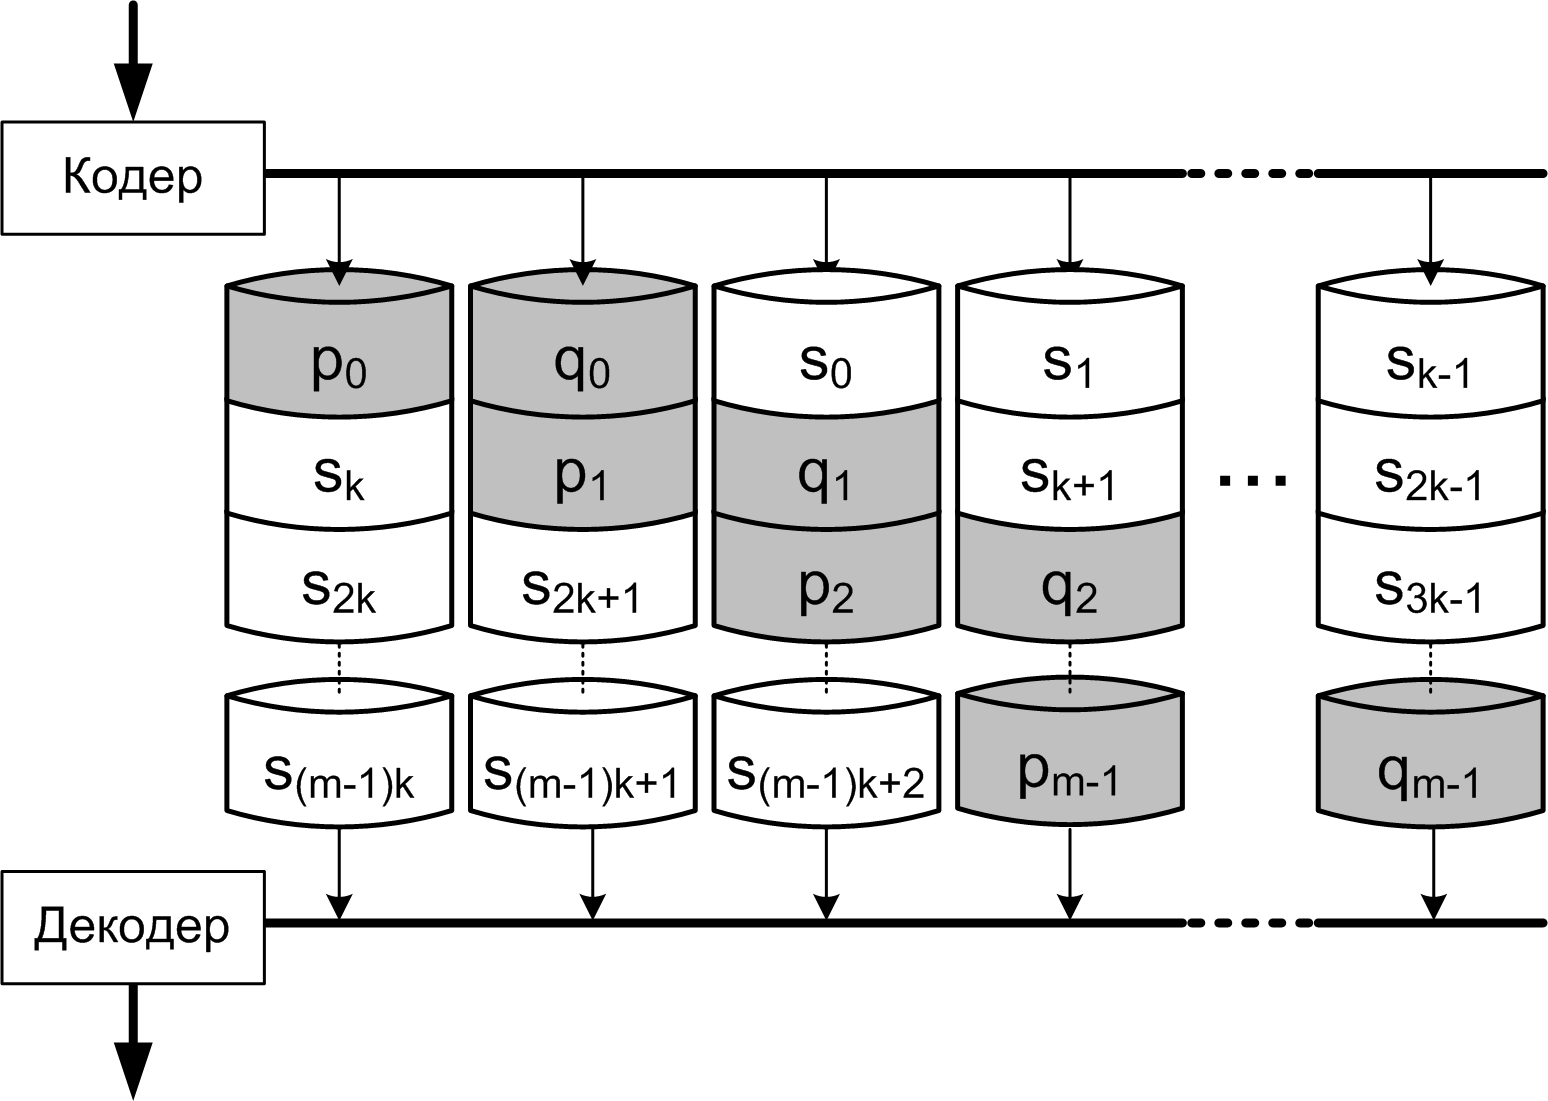
\includegraphics[width=.8\textwidth]{pict/raid6} } 
            \caption{RAID 6}\label{pict:raid6}
        \end{center}
    \end{figure} 
    \mode<article>{см. рис. \ref{pict:raid6}}
\end{frame}

RAID 6 похож на RAID 5: данные разбиваются на блочном уровне, но для повышения отказоустойчивости используется дополнительная контрольная сумма. Рассчет дополнительной контрольной суммы опирается на теорию групп (арифметика полиномов).

Минимальное количество дисков: $n=4$; Эффективность использования дискового пространства: $\frac{n-2}{n}$.

Преимущества:
\begin{itemize}
    \item высокая отказоустойчивость (работа после выхода из строя двух дисков);
    \item достаточно высокая скорость обработки запросов;
    \item относительно малые накладные расходы для реализации избыточности.
\end{itemize}

Недостатки:
\begin{itemize}
    \item сложная реализация;
    \item медленное восстановление данных;
    \item скорость записи данных ниже, чем в RAID 5.
\end{itemize}

%TODO raid 6

\[
    p=\bigoplus_{j=0}^{k-1}s_{j}; q=\bigoplus_{j=0}^{k-1}g^js_{j},
\]
где $g$ --- образующий многочлен (т.е. степенью $g^i$ можно представить любой элемент поля $GF(2^8)=F_2[X]/(X^8+x^4+X^3+X^2+1)$).

Более точно, в соответствии с рисунком \ref{pict:raid6}:
\[
    p_i=\bigoplus_{j=0}^{k-1}s_{ki+j}; q_i=\bigoplus_{j=0}^{k-1}g^js_{ki+j}.
\]


\end{document}